\chapter{Ergebnisse}


\section{Relacsauswertung}

\subsection{"Ubersicht}

Abbildung \ref{fig:overview1} zeigt die gesammelten Leistungen von Fisch 1 �ber den gesamten Hauptversuch. Zun�chst wurde der Fisch an 19 Versuchstagen mit je 10 Durchl�ufen pro Versuchstag mit Stimuli der Signalst�rke ein Millivolt trainiert. An den folgenden elf Versuchstagen wurde er dann auf eine Amplitude von zwei Millivolt trainiert. Die Zahlen, welche sich �ber den einzelnen Balken befinden, geben an, bei wie vielen Durchl�ufen pro Versuchstag eine Entscheidung getroffen wurde. Steht keine Zahl �ber dem Balken, hat sich der Fisch bei allen zehn Versuchsdurchl�ufen entschieden. Links neben der Grafik, welche die Richtige Entscheidung von Fisch 1 pro Versuchstag anzeigt, findet sich ein Boxplot. Dieser zeigt die Verteilung der Leistungen von Fisch eins �ber den gesamten Hauptversuchszeitraum. Fisch 1 hat dabei mit einem Median von ??? abgeschnitten. Der Binomialtest gibt eine Wahrscheinlichkeit, daf�r dass es sich bei dieser Verteilung um einen Zufall handelt von ??? an (P-Wert). Die Leistungen von Fisch 1 bei einem Millivolt und bei zwei Millivolt werden im Folgenden noch genauer analysiert. 

Abbildung \ref{fig:overview2} zeigt die �bersicht des gesamten Hauptversuchs analog zu Abbildung \ref{fig:overview1} f�r Fisch 2. Im Unterschied zu Abbildung \ref{fig:overview1} wurde bei Fisch 2 noch ein weiteres Experiment durchgef�hrt: Ab dem 06.10.2015 wurden bei Fisch 2 der S+ und S- Stimulus vertauscht. Genaueres wird in der folgenden Analyse folgen.

\begin{figure}[ht]
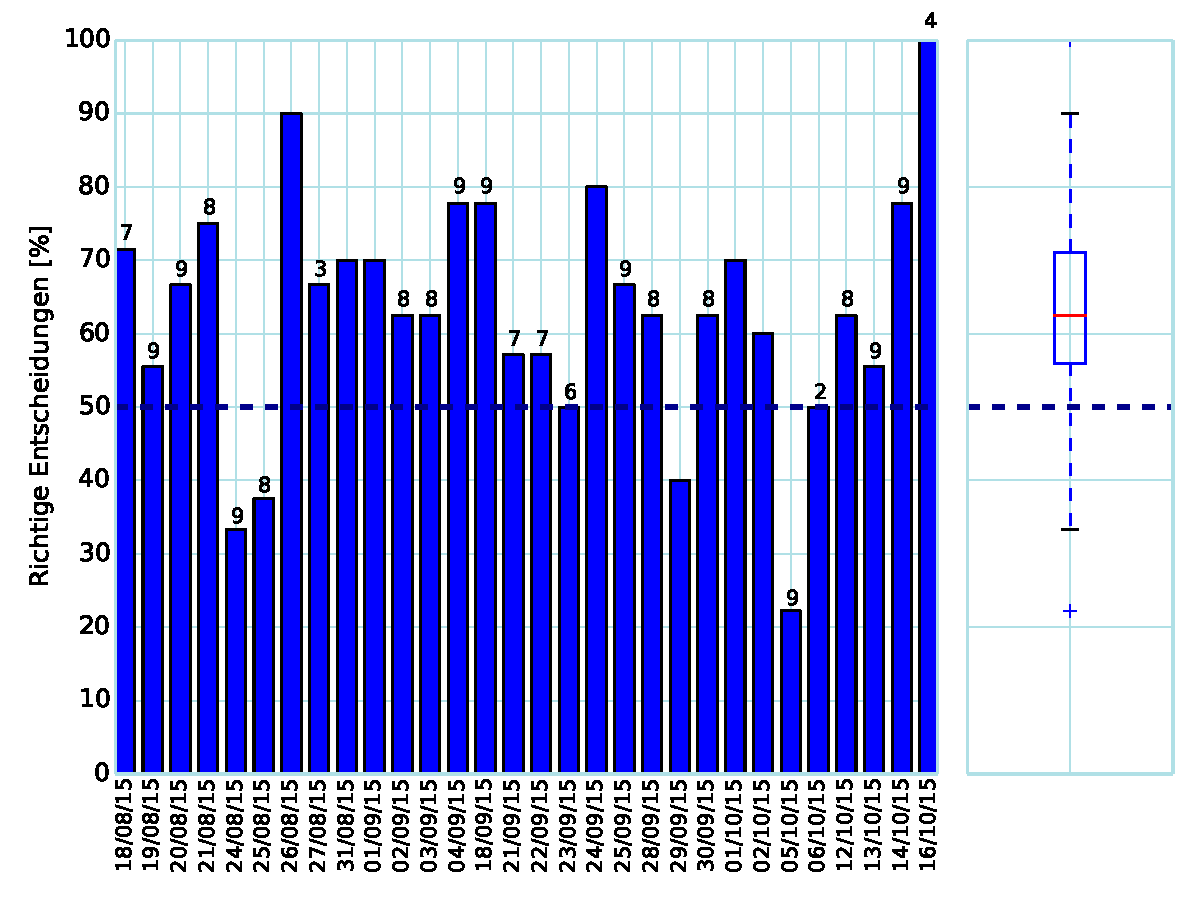
\includegraphics[height=8.5cm]{Abbildungen/Overview1}
\caption{\label{fig:overview1}Overview Fisch 1 mit Boxplot}
\end{figure}

\begin{figure}[ht]
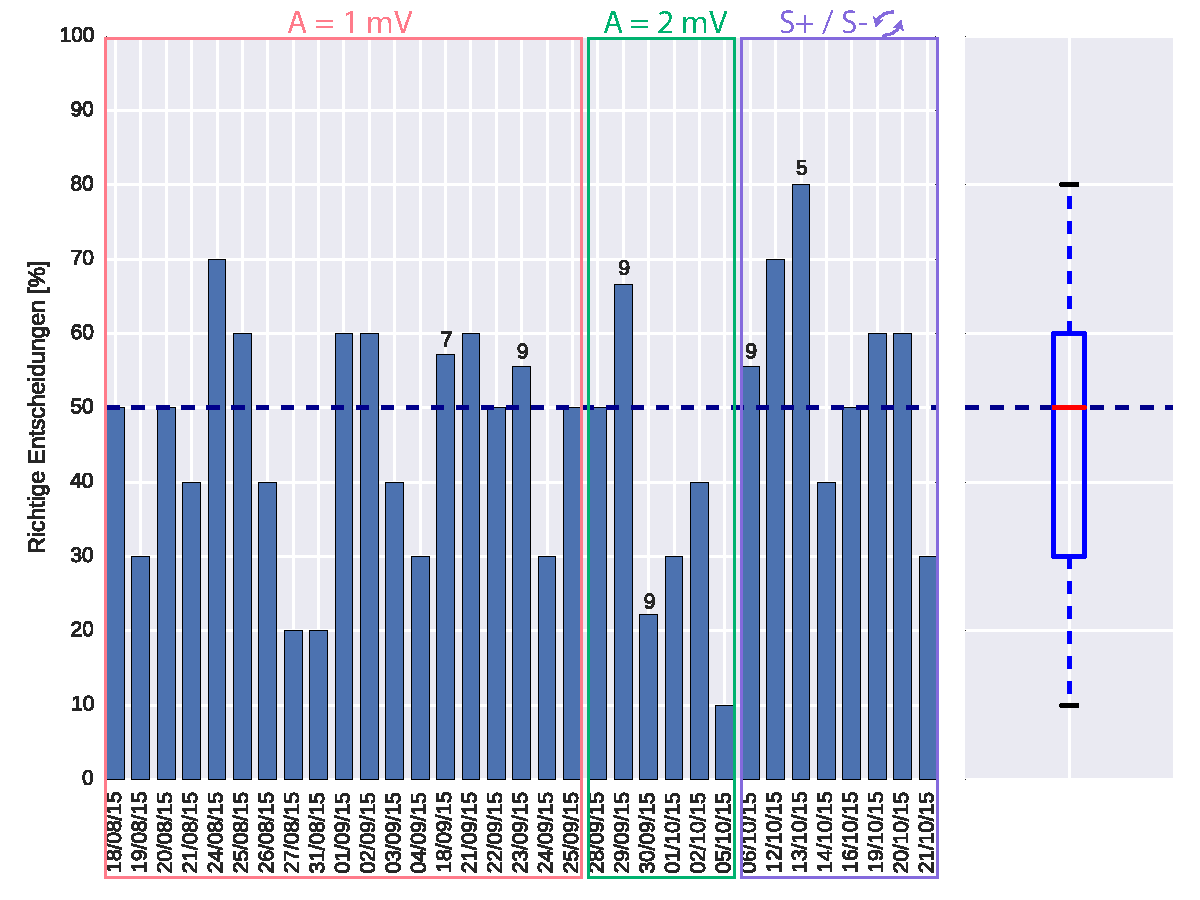
\includegraphics[height=8.5cm]{Abbildungen/Overview2}
\caption{\label{fig:overview2}Overview Fisch 2 mit Boxplot}
\end{figure}

\subsection{Amplitude 1 Millivolt vs. Amplitude 2 Millivolt}

Fisch 1 schnitt beim Trainig bei einer Amplitude mit einer gewichteten Mittleren Leistung von ??? ab. Ein Binomialtest erbrachte hierf�r einen P-Wert von ???. Wie in Abbildung \ref{fig:amplitude1_1} zu sehen lag Fisch 1 bei einem mittleren Median von ???.
\begin{figure}[ht]
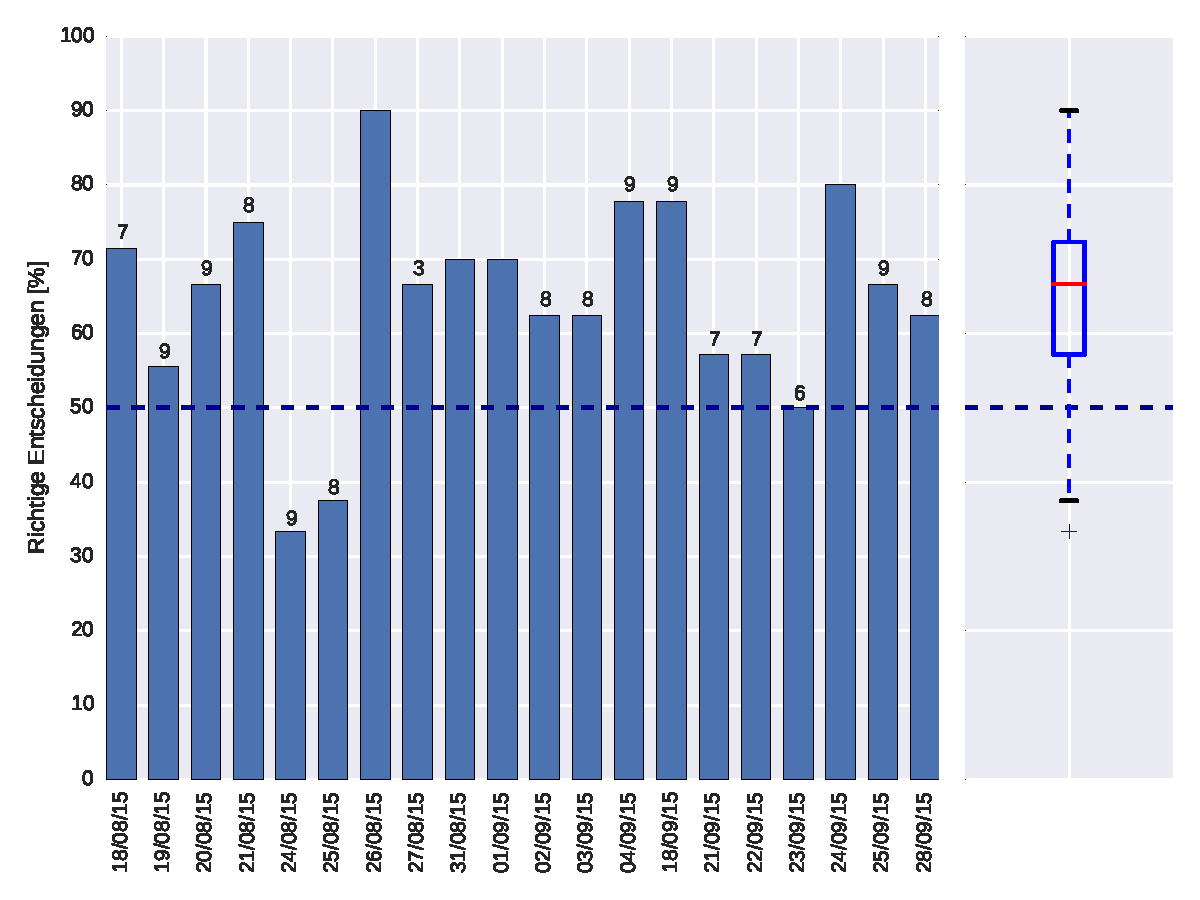
\includegraphics[height=8.5cm]{Abbildungen/Performanceamplitude_is_one2015albi02}
\caption{\label{fig:amplitude1_1}Links: Die Leistung von Fisch 1 bei einer Stimulusamplitude von einem Millivolt. Auf der X-Achse sind die jeweiligen Daten der Versuchstage abgebildet, auf der Y-Achse sind die richtigen Entscheidungen des Fisches in Prozent zu sehen. Rechts: Boxplot, der die Verteilung der Leistungen des Fisches zeigt.}
\end{figure}


Fisch 2 hingegen erreichte beim Training mit Stimuli von einem Millivolt lediglich Leistungen von ??? im Median. Der Binomialtest ergab hierbei ???. Um zu �berpr�fen, ob die Versuchstiere auf eine h�here Signalintensit�t anders reagieren, wurde der Stimulus auf zwei Millivolt verdoppelt.
\begin{figure}[ht]
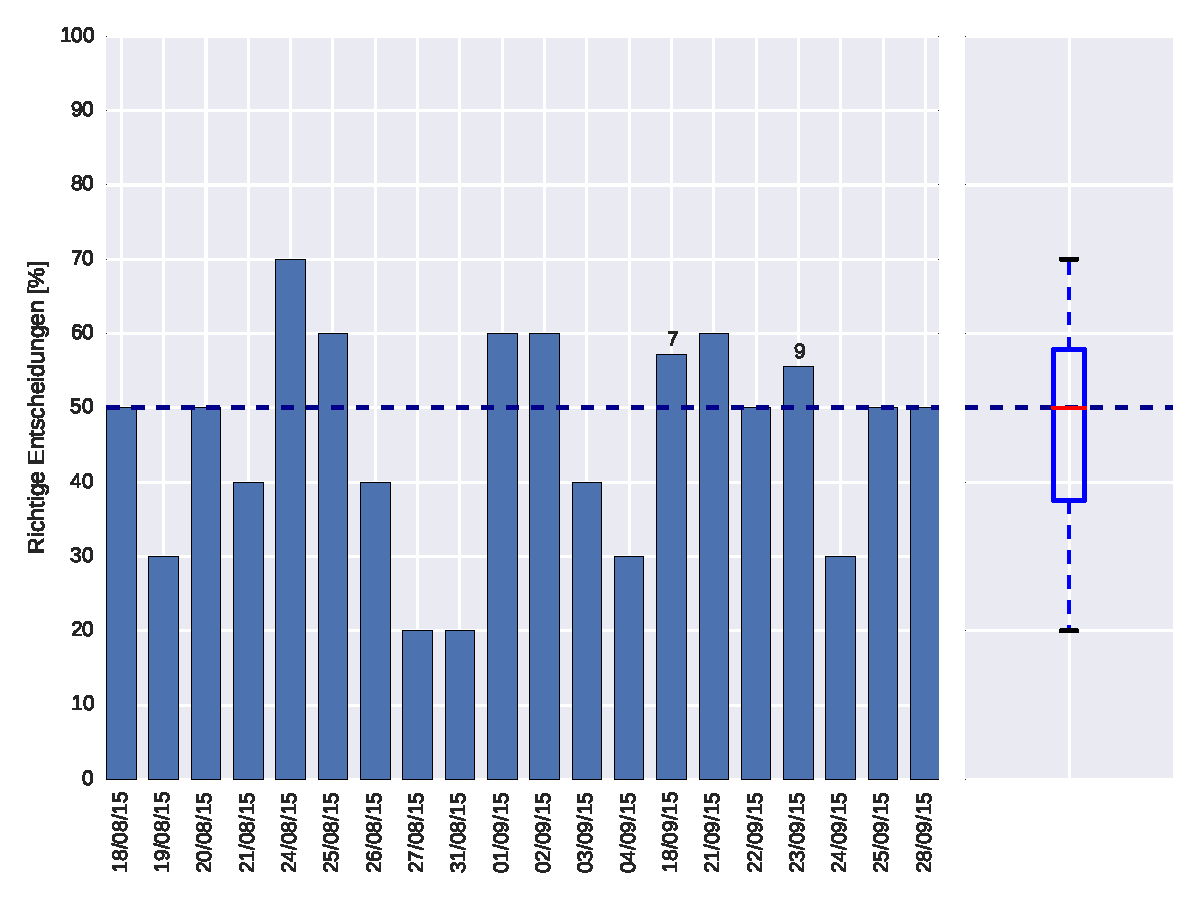
\includegraphics[height=8.5cm]{Abbildungen/Performanceamplitude_is_one2015albi01} \caption{\label{fig:amplitude1_2}Links: Die Leistung von Fisch 2 bei einer Stimulusamplitude von einem Millivolt. Auf der X-Achse sind die jeweiligen Daten der Versuchstage abgebildet, auf der Y-Achse sind die richtigen Entscheidungen des Fisches in Prozent zu sehen. Rechts: Boxplot, der die Verteilung der Leistungen des Fisches zeigt.}
\end{figure}

Abbildung \ref{fig:amplitude2_1} zeigt die Leistungen von Fisch 1 bei einer Amplitude von 2 mV. Hierbei lag der Median bei ??? und der Binomialtest ergab einen P-Wert von ???.

\begin{figure}[ht]
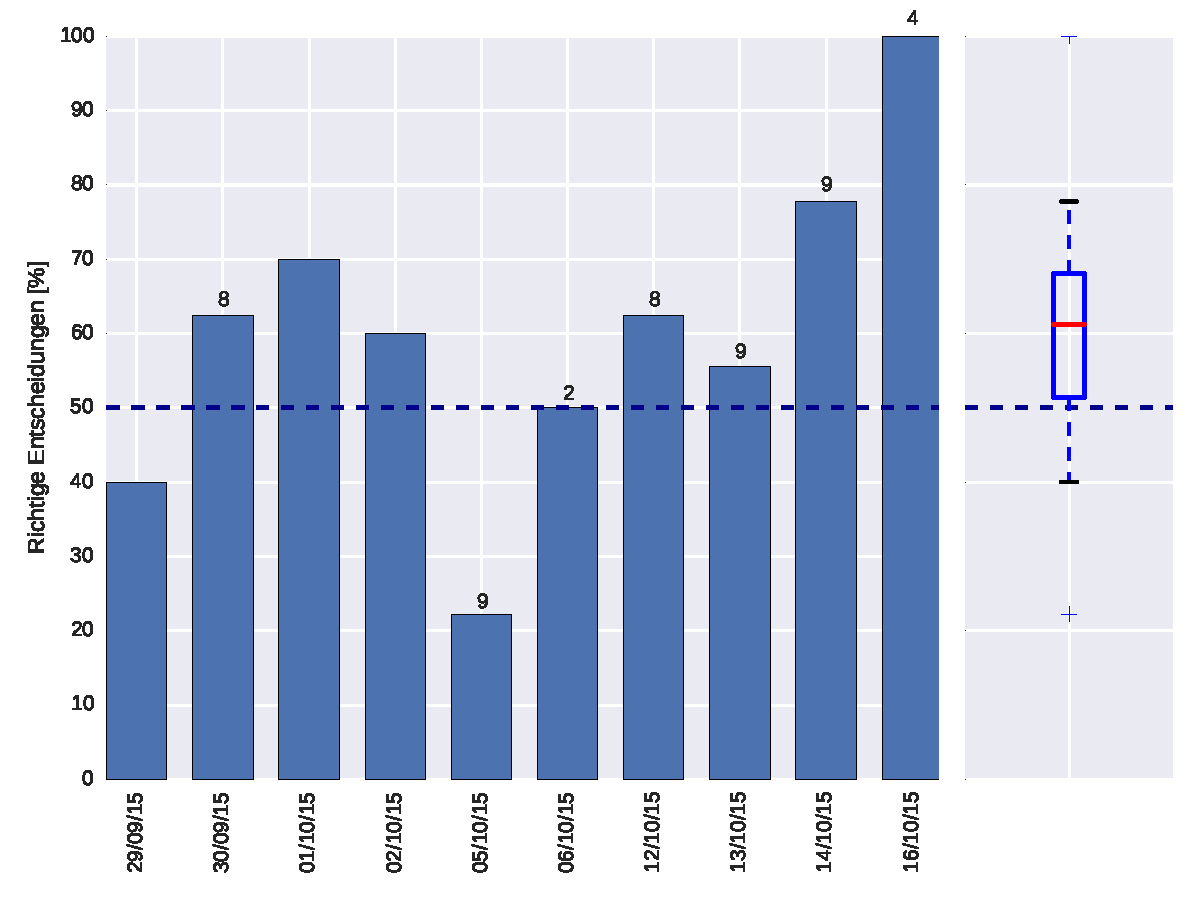
\includegraphics[height=8.5cm]{Abbildungen/Performanceamplitude_is_two2015albi02}
\caption{\label{fig:amplitude2_1} Links: Die Leistung von Fisch 1 bei einer Stimulusamplitude von zwei Millivolt. Auf der X-Achse sind die jeweiligen Daten der Versuchstage abgebildet, auf der Y-Achse sind die richtigen Entscheidungen des Fisches in Prozent zu sehen. Rechts: Boxplot, der die Verteilung der Leistungen des Fisches zeigt.}
\end{figure}

Fisch 2 ging in seiner Performance nach der Amplituden�nderung noch weiter runter wie in Abbildung \ref{fig:amplitude2_2} zu sehen. Der Median betrug lediglich ??? und der Binomialtest ergab einen Wert von ???.

\begin{figure}[ht]
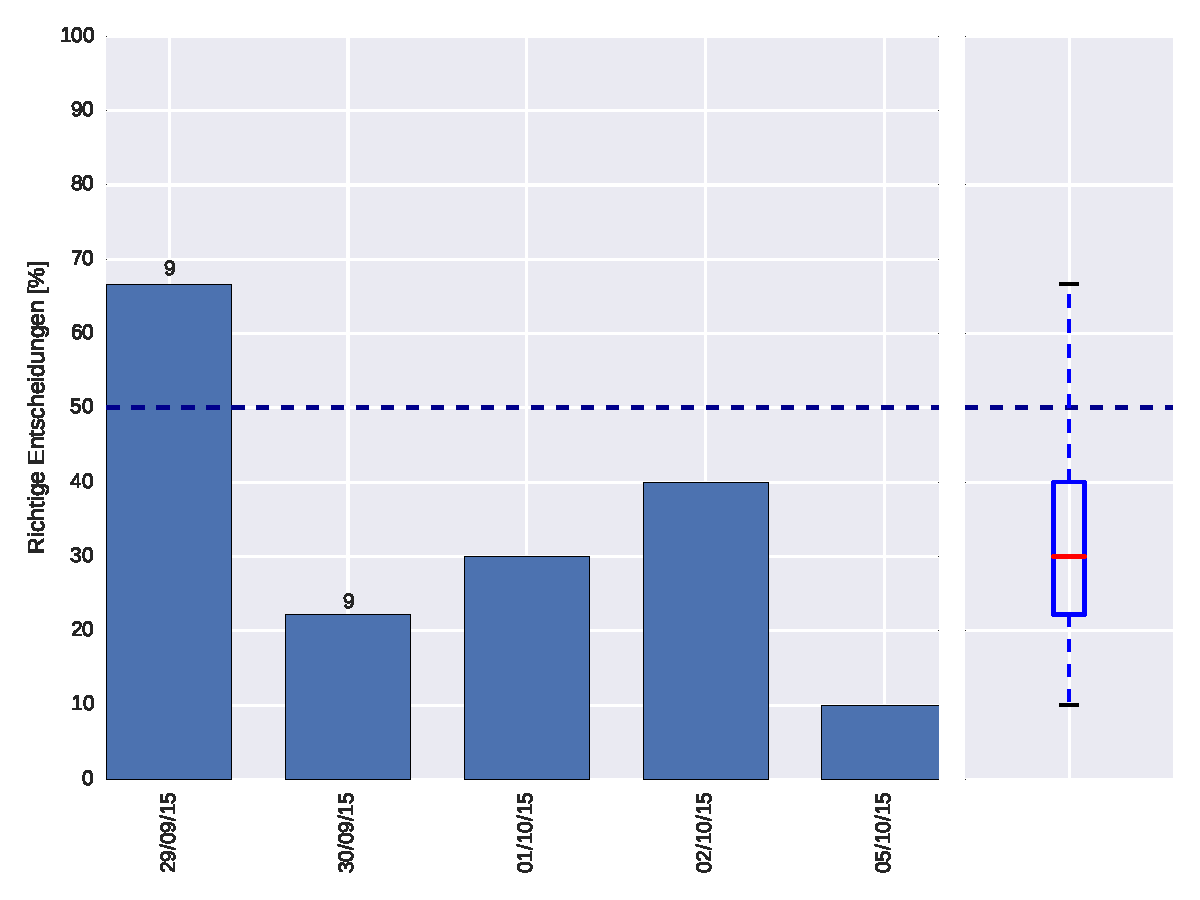
\includegraphics[height=8.5cm]{Abbildungen/Performanceamplitude_is_two2015albi01}
\caption{\label{fig:amplitude2_2} Links: Die Leistung von Fisch2 bei einer Stimulusamplitude von zwei Millivolt. Auf der X-Achse sind die jeweiligen Daten der Versuchstage abgebildet, auf der Y-Achse sind die richtigen Entscheidungen des Fisches in Prozent zu sehen. Rechts: Boxplot, der die Verteilung der Leistungen des Fisches zeigt.}
\end{figure}

Abbildung \ref{fig:getauscht} zeigt die Leistungen von Fisch 2, nachdem der S+ und der S- Stimulus vertauscht worden waren. Der neue S+ Stimulus war demnach ein eigenmanniaartiges Signal mit einer Frequenz von 60 Hertz, w�hrend der neue S- Stimulus nun ein einfaches Signal mit einer Frequenz von 60 Hertz war.

\begin{figure}[ht]
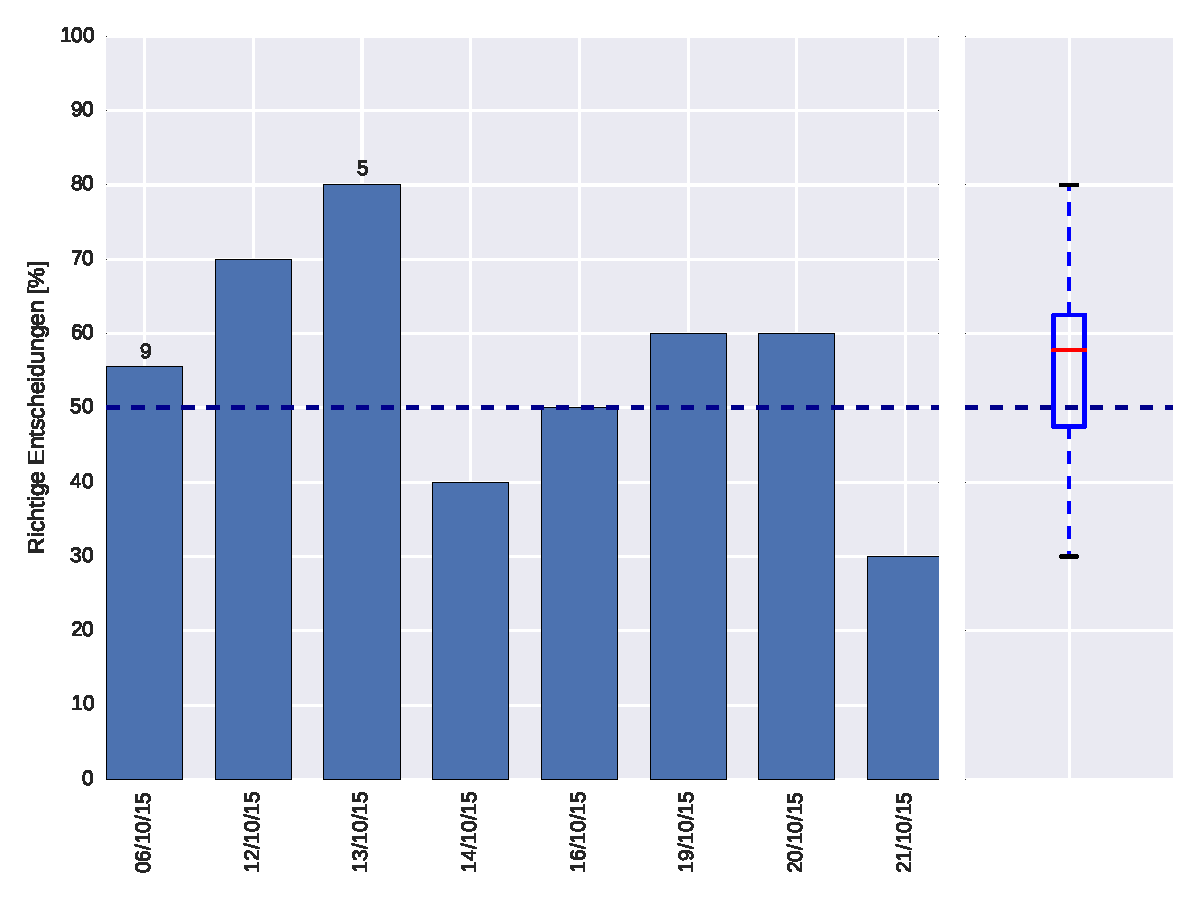
\includegraphics[height=8.5cm]{Abbildungen/performance_chap_changed_stimuli2015albi01}
\caption{\label{fig:getauscht}Fisch 2 vertauschte Stimuli mit Boxplot}
\end{figure}


\section{Videotrackingauswertung}
Jeder Versuchsdurchlauf wurde beim Hauptversuch auf Video aufgenommen. Dabei wurde das Video gestartet, bevor die Startbox ge�ffnet wurde. Beendet wurde das Video bevor die Belohnung stattfand oder der Fisch zur�ck in die Startbox gef�hrt wurde.
Die Videodateien wurden dann wie bereits im Kapitel Datenanalyse erl�utert mit Hilfe eines Trackingprogramms analysiert.


%%%%%% IN DAS TRACKINGBILD NOCH BESCHRIFTUNGEN EINF�GEN MIT ELEKTRODE 1; ELEKTRODE2, 	TOR ZUR STARTBOX




\subsection{Beispielvideo}

Anhand eines Beispielvideos wird im Folgenden das Vorgehen bei der Videotrackingauswertung gezeigt:

\begin{figure}[ht]
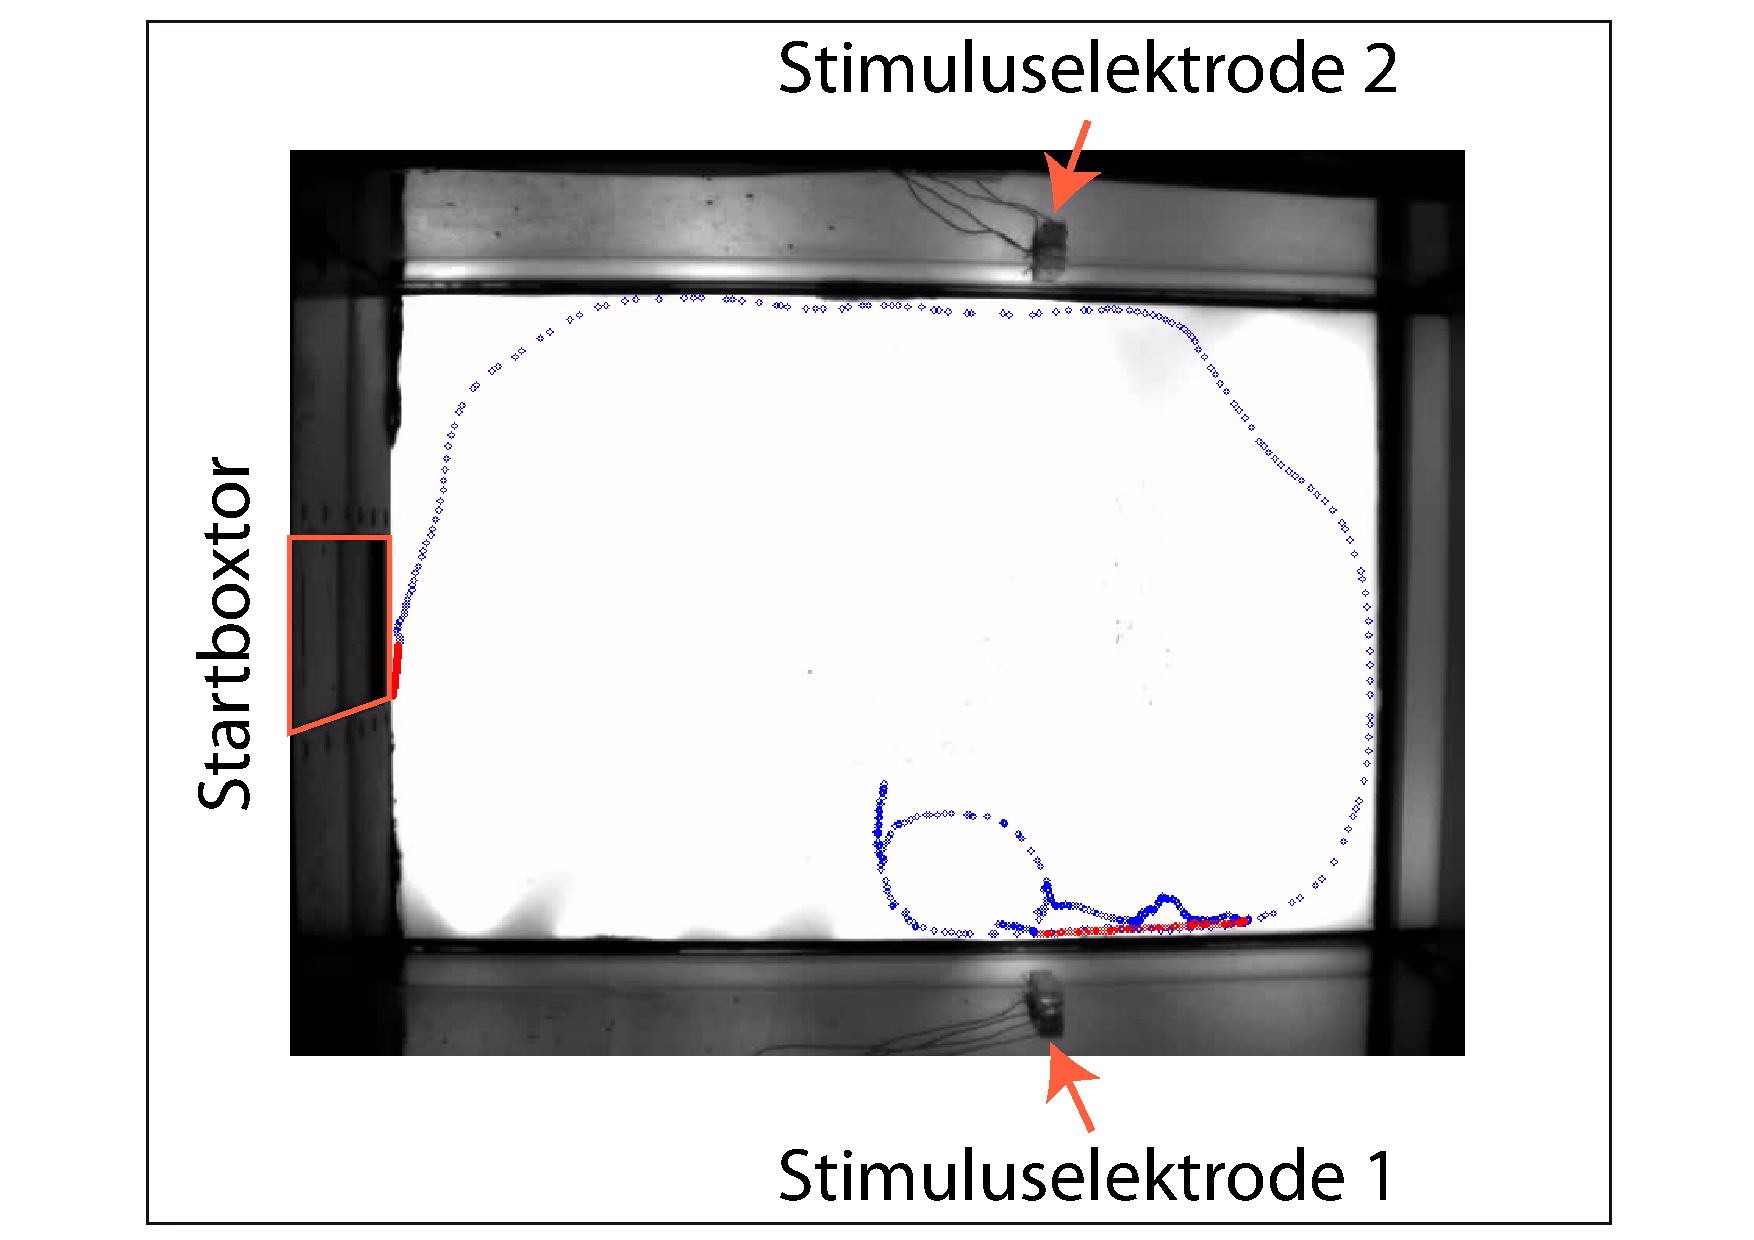
\includegraphics[height=8.5cm]{Abbildungen/2015-08-18_1_OV_path}
\caption{\label{fig:path}Trackingbild. Der blaue Pfad zeigt die sicher Position des Fisches an. Bei den roten Punkten, hat das Trackingprogramm den Fisch kurzzeitig verloren, diese sind gesch�tzte Positionen des Trackingprogramms.}
\end{figure}

Zun�chst wurde jedes Video einzeln mit dem Trackingprogramm getrackt, dabei wurden die X und Y Position im Versuchsbecken und die Orientierung des Versuchstiers f�r jedes Videoframe in Listen gespeichert. Au�erdem wurde eine Graphik erstellt, welche den zur�ckgelegten Weg des Fisches zeigt (siehe Abb. \ref{fig:path}).
In dem in Abbildung \ref{fig:path} gezeigten Beispiel war Elektrode 1, die belohnte Elektrode, die den S+ Stimulus abgab. Das Versuchstier war in diesem Beispiel Fisch 2.
Anhand des blauen Pfades ist zu sehen, das Fisch 2 zun�chst an der falschen Elektrode (Elektrode 2) vorbei geschwommen ist und sich schlie�lich f�r Elektrode 1 entschieden hat.
Im Folgenden soll gezeigt werden, worauf diese Behauptung beruht.

Zun�chst konnte so zum Beispiel zun�chst bei jedem einzelnen Video die Entfernungen zu Elektrode 1 und Elektrode 2 berechnet werden. Abbildung \ref{fig:distanzen} zum Beispiel zeigt f�r das Videobeispiel die Distanzen zu Elektrode 1 und zu Elektrode 2. 


%%%%%%%%%%%BEIM ORIENTIERUNGS BILD UMBEDINGT NOCH DAS GANZE BECKEN ZEIGEN UND EVTL TRACKINGBILD DRUNTER LEGEN%%%%%%%%%%%

\begin{figure}[ht]
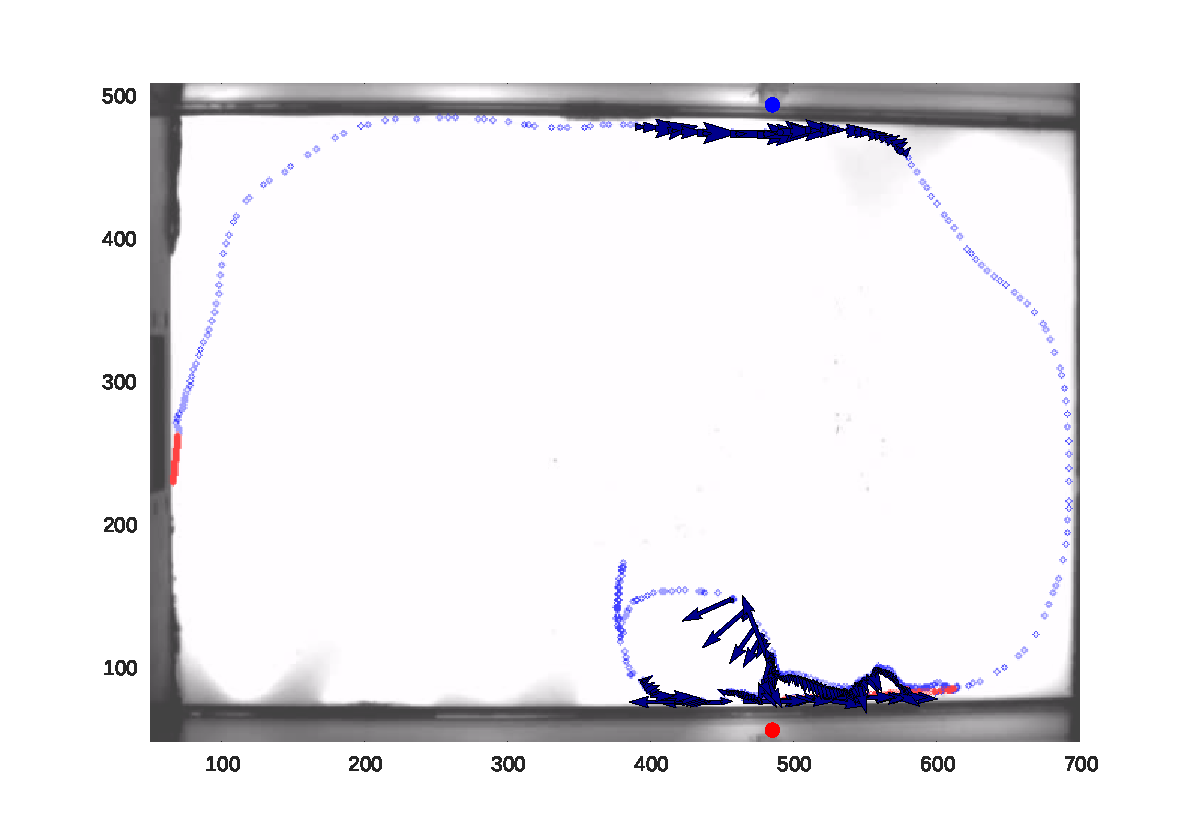
\includegraphics[height=8.5cm]{Abbildungen/Orientierung_2015-08-18_1}
\caption{\label{fig:orientierung}Orientierung}
\end{figure}

\begin{figure}
\subfigure[Distanz zu Elektrode 1 �ber die Zeit]{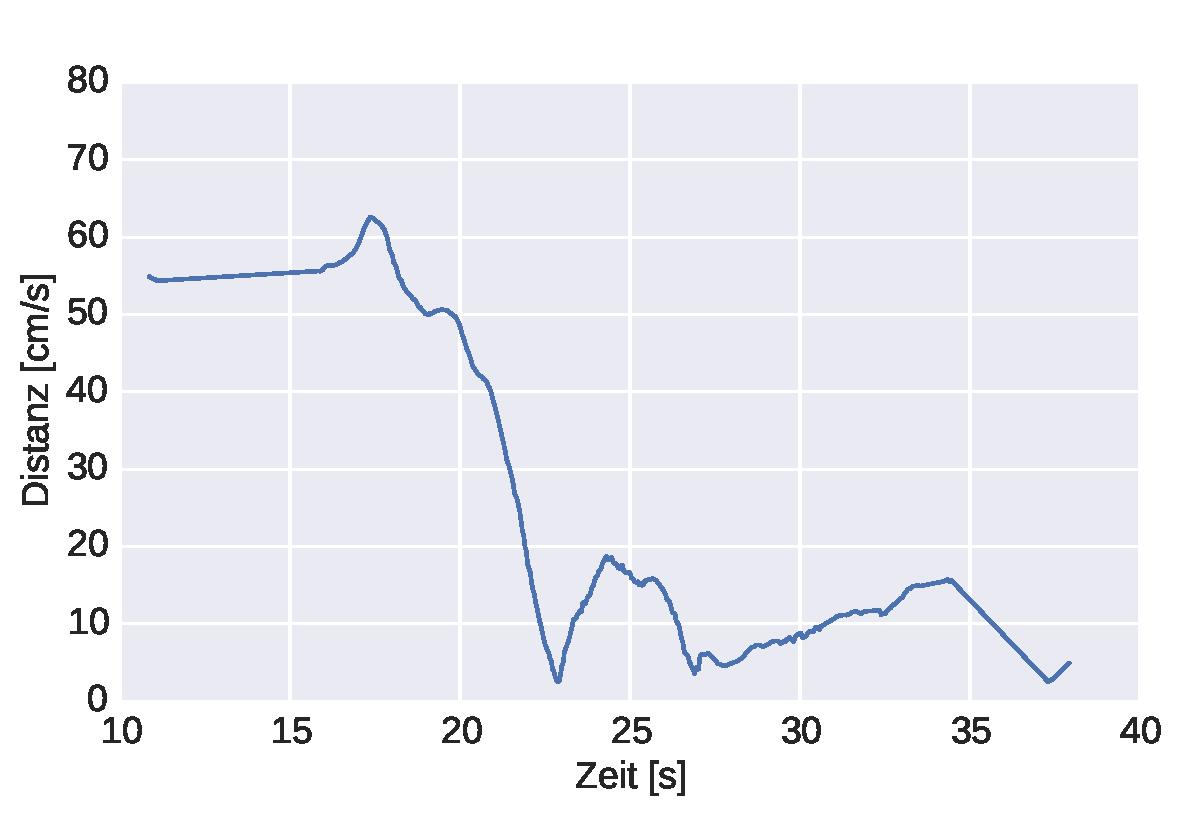
\includegraphics[height=6cm]{Abbildungen/distance_time_plot_2015-08-18_1_electrode1}}
\subfigure[Distanz zu Elektrode 2 �ber die Zeit]{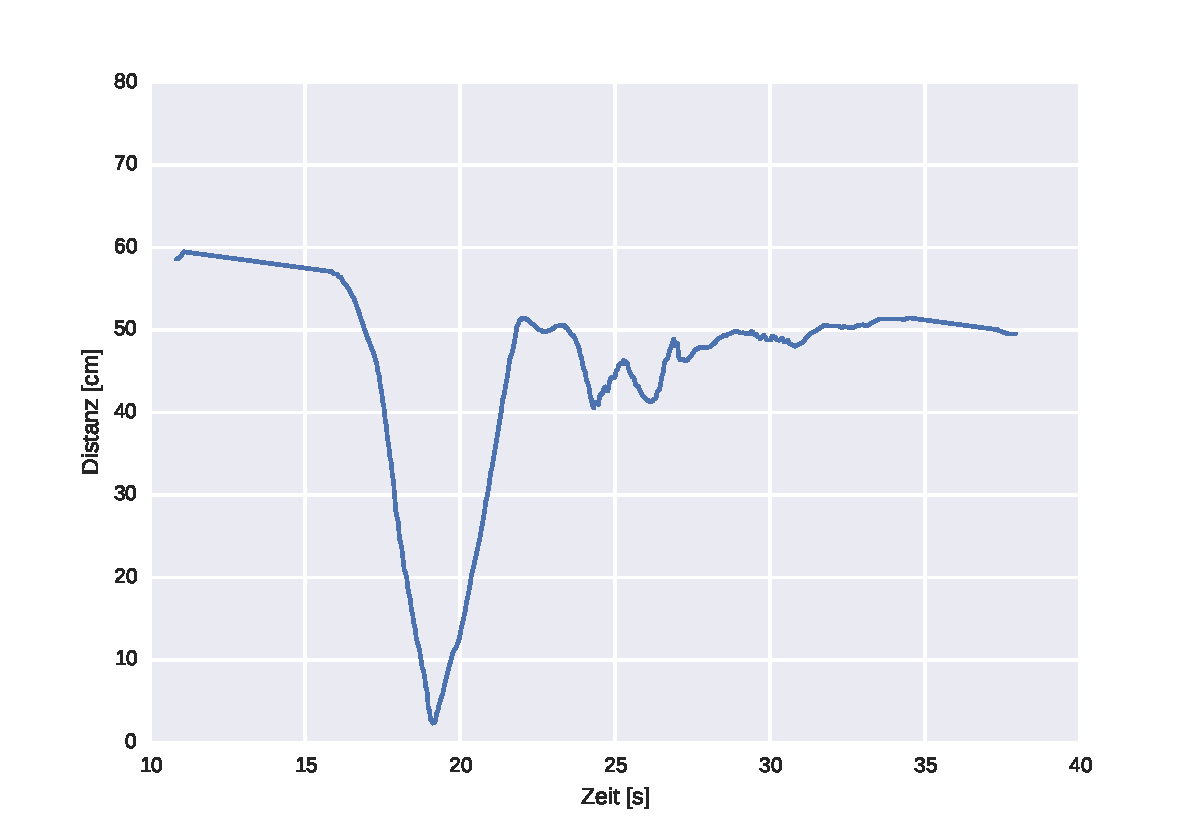
\includegraphics[height=6cm]{Abbildungen/distance_time_plot_2015-08-18_1_electrode2}}
\caption{\label{fig:distanzen}Versuchsaufbau}
\end{figure}

\subsection{Video�bergreifende Auswertung}

\begin{figure}[ht]
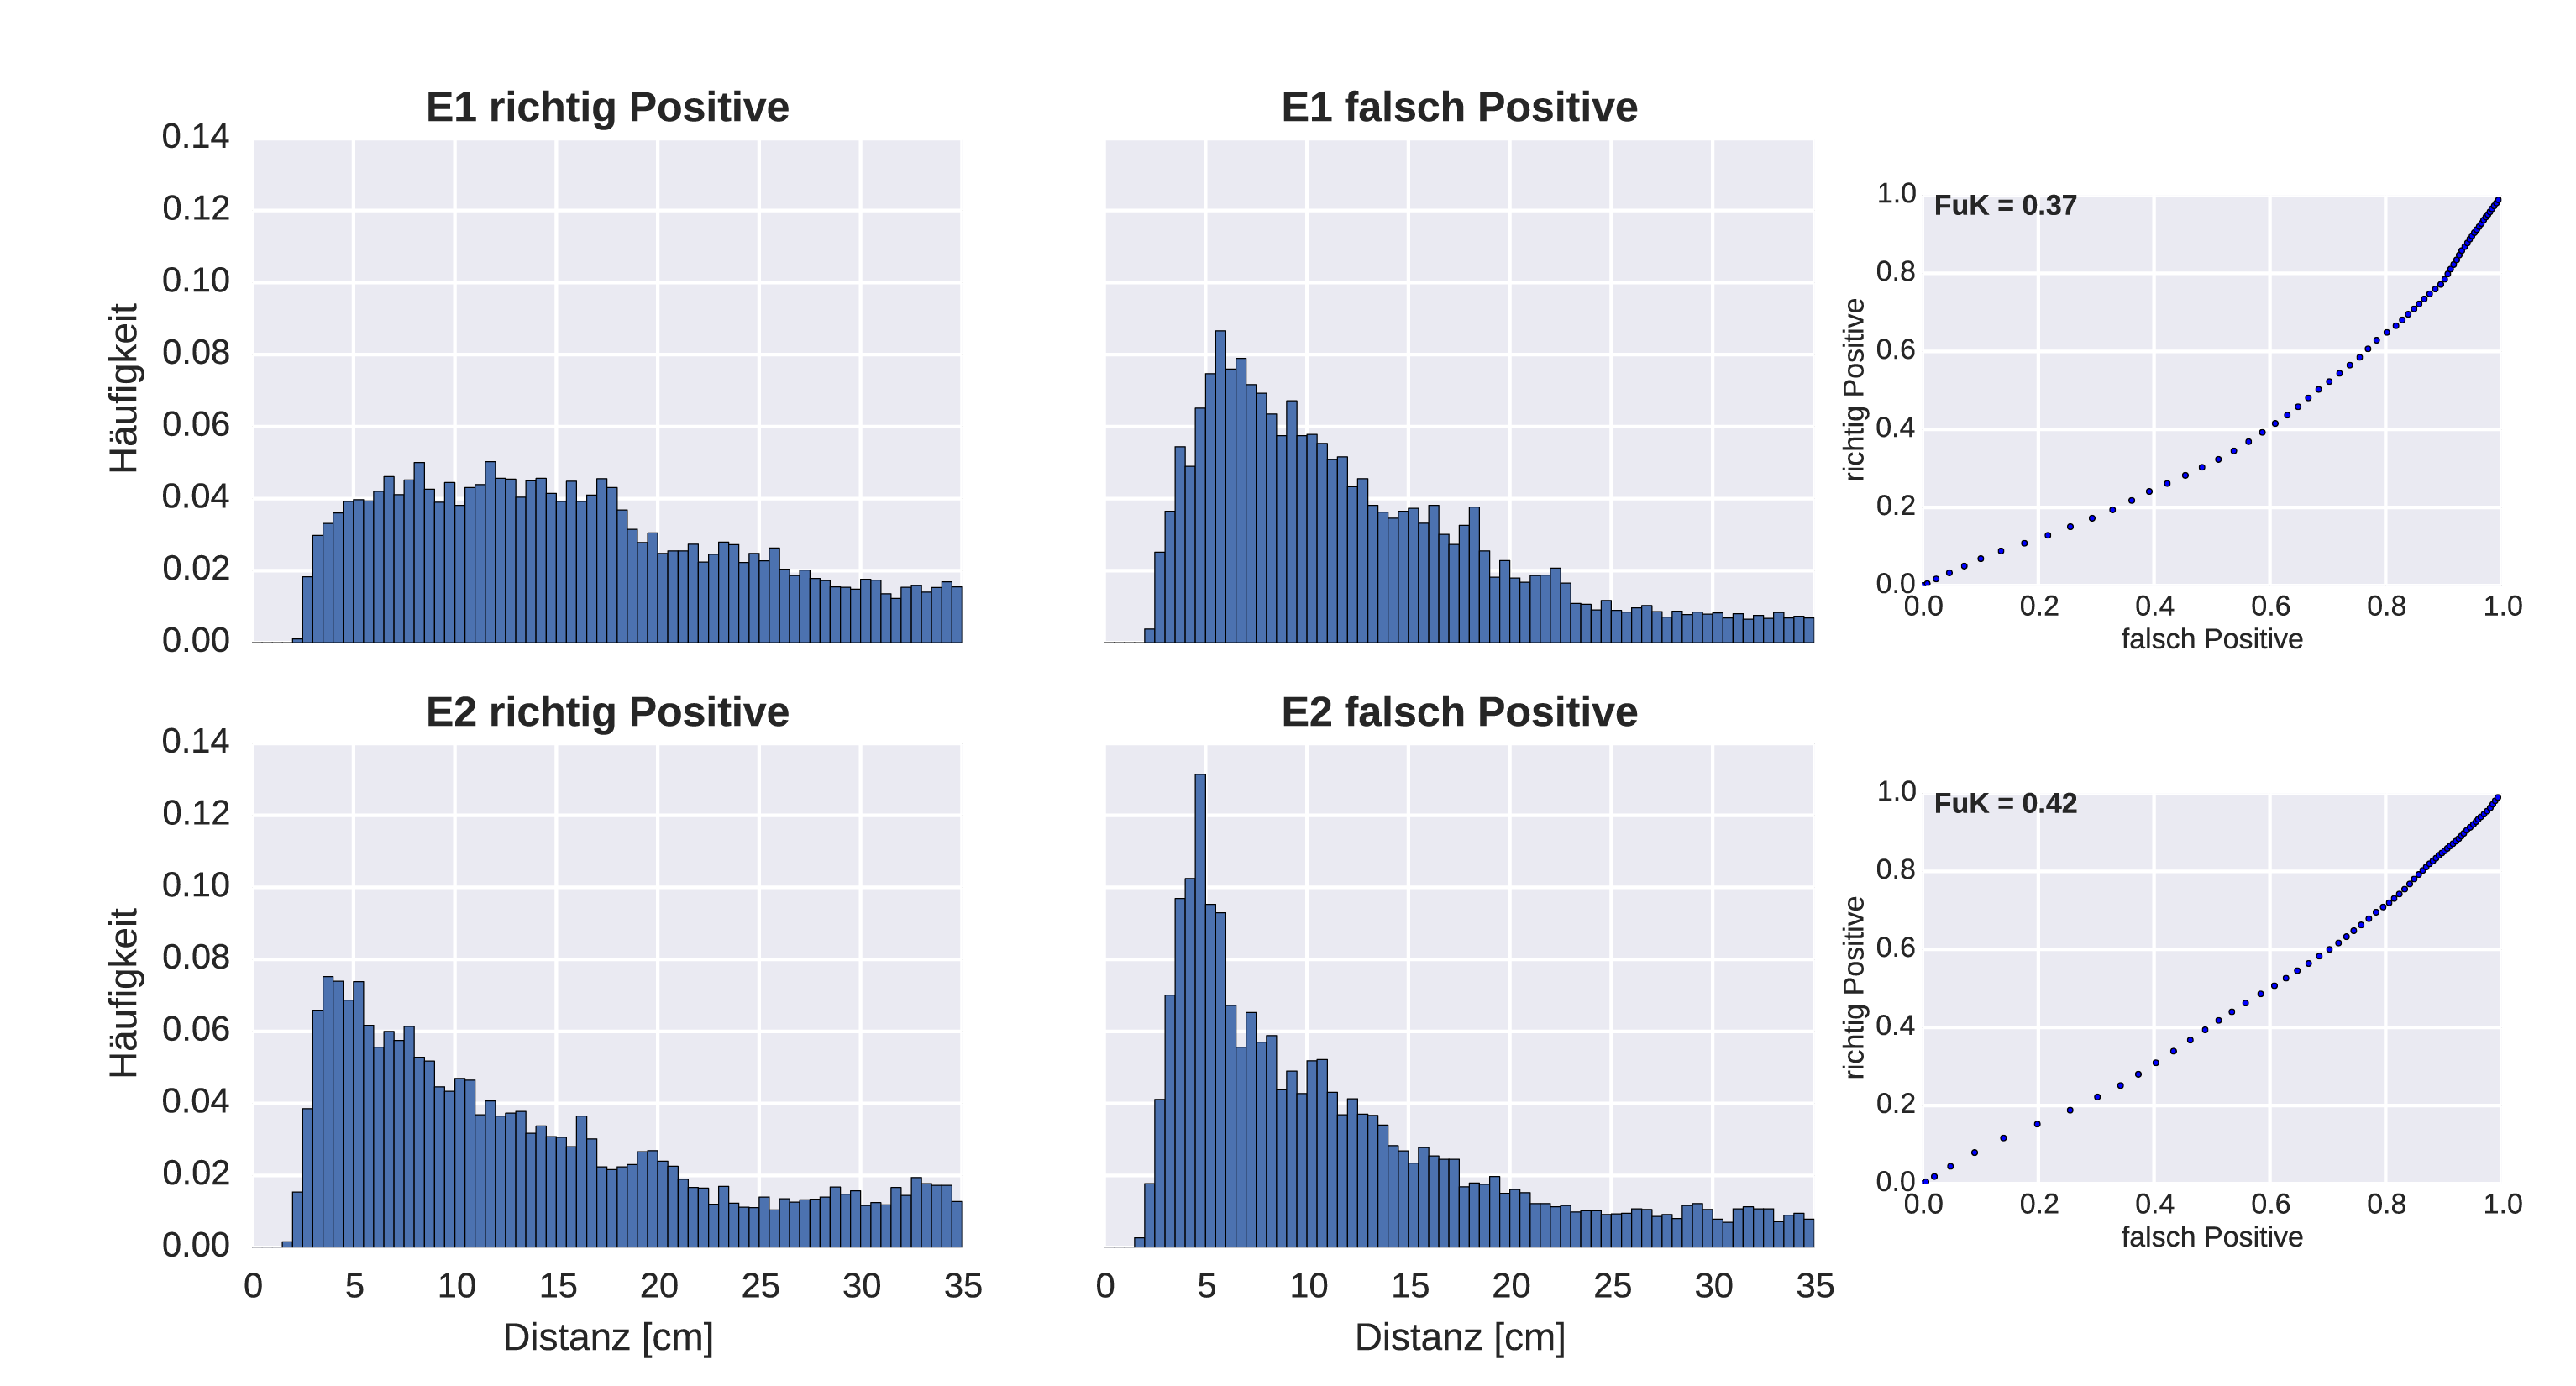
\includegraphics[height=10.5cm]{Abbildungen/Histogramm_Elektrodendistanzen_mit_Fischentscheidung2015albi02}
\caption{\label{fig:histodistanzen_entscheidung1}Fisch 1 Histogramme zur Distanz zu den Elektroden mit fischentscheidung}
\end{figure}


\begin{figure}[ht]
\subfigure[Roc Kurve Elektrode 1]
{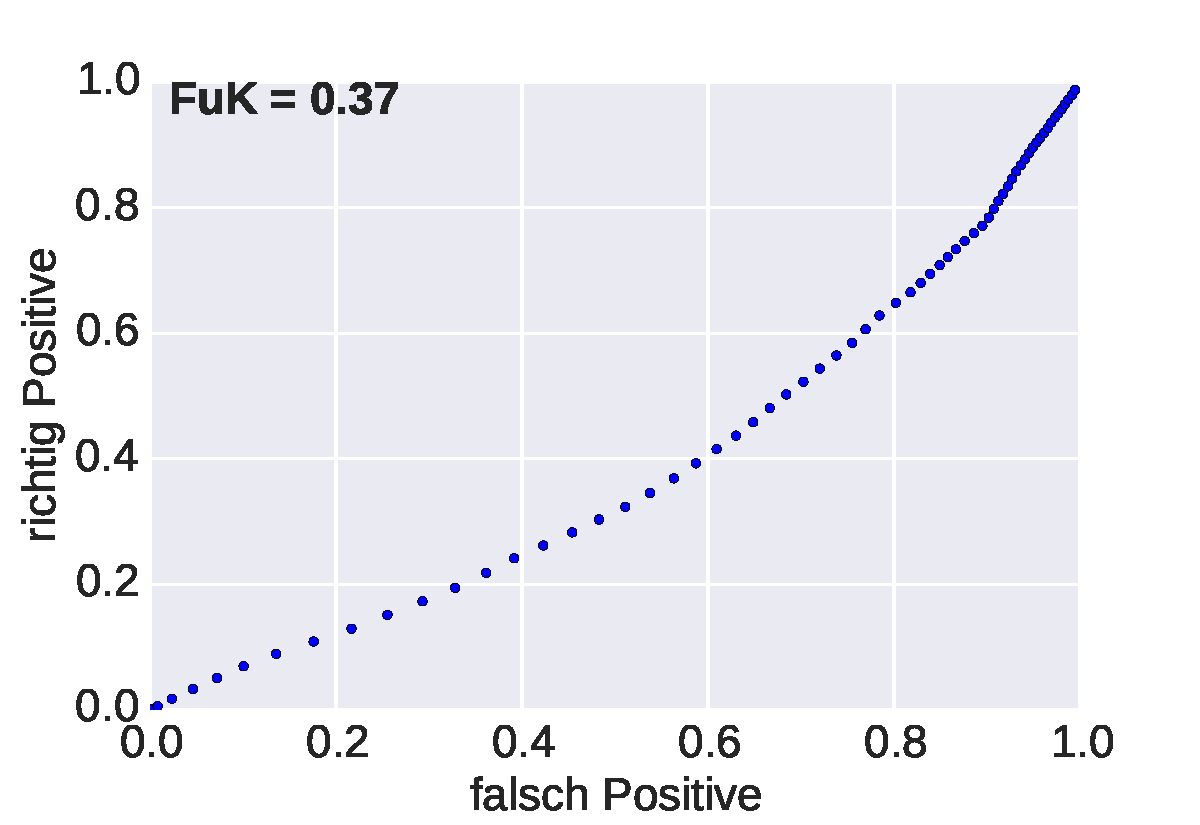
\includegraphics[height=6cm]{Abbildungen/roc_curve_E1Distanz2015albi02}}
\subfigure[Roc Kurve Elektrode 2]
{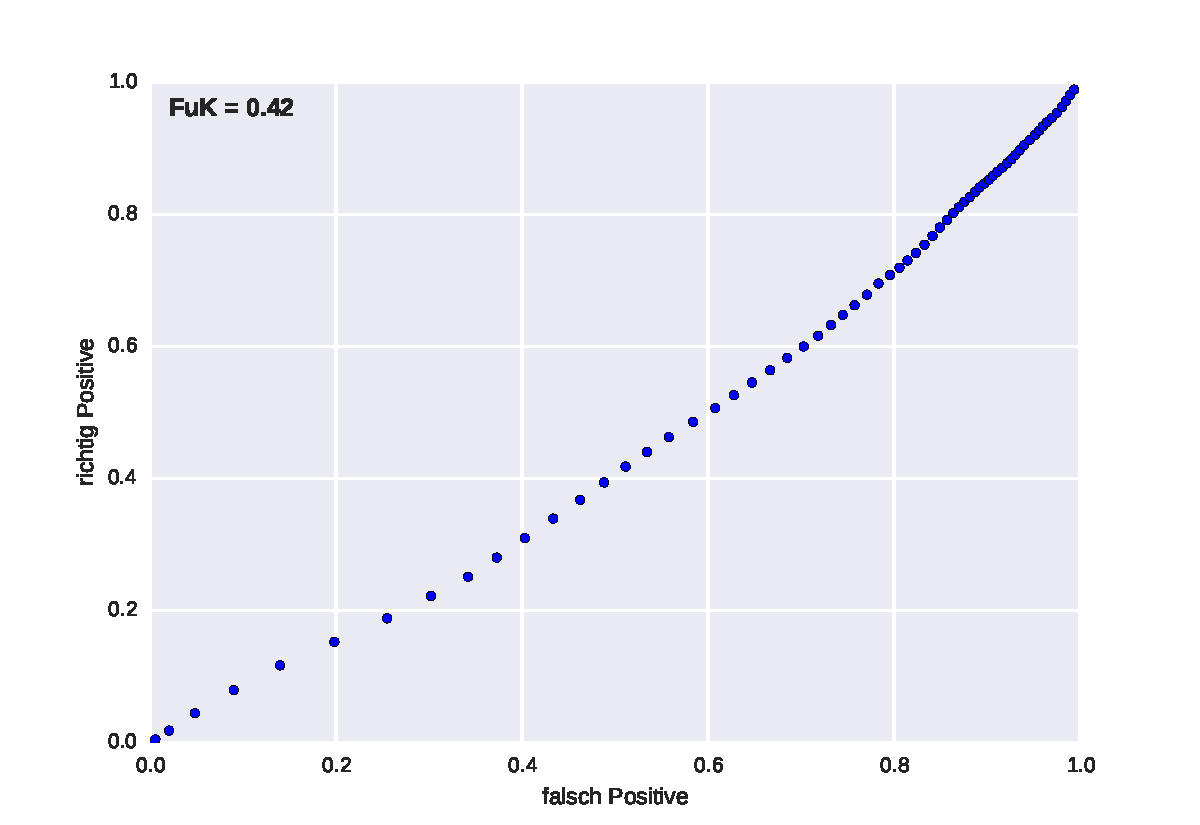
\includegraphics[height=6cm]{Abbildungen/roc_curve_E2Distanz2015albi02}}
\caption{\label{fig:roc_distanzen_entscheidung1}Roc Kurven dazu von Fisch 1}
\end{figure}


\begin{figure}[ht]
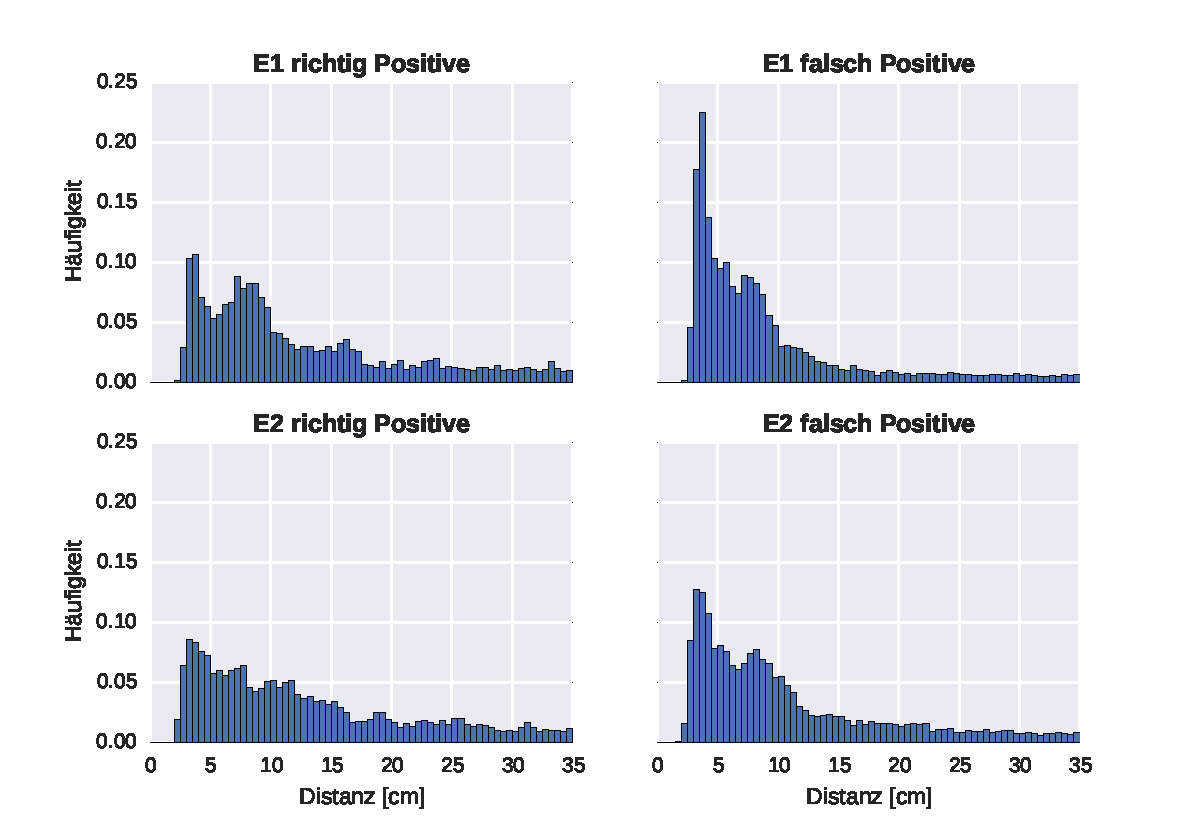
\includegraphics[height=10.5cm]{Abbildungen/Histogramm_Elektrodendistanzen_mit_Fischentscheidung2015albi01}
\caption{\label{fig:histodistanzen_entscheidung2}Fisch 2 Histogramme zur Distanz zu den Elektroden mit fischentscheidung}
\end{figure}


\begin{figure}[ht]
\subfigure[Roc Kurve Elektrode 1]
{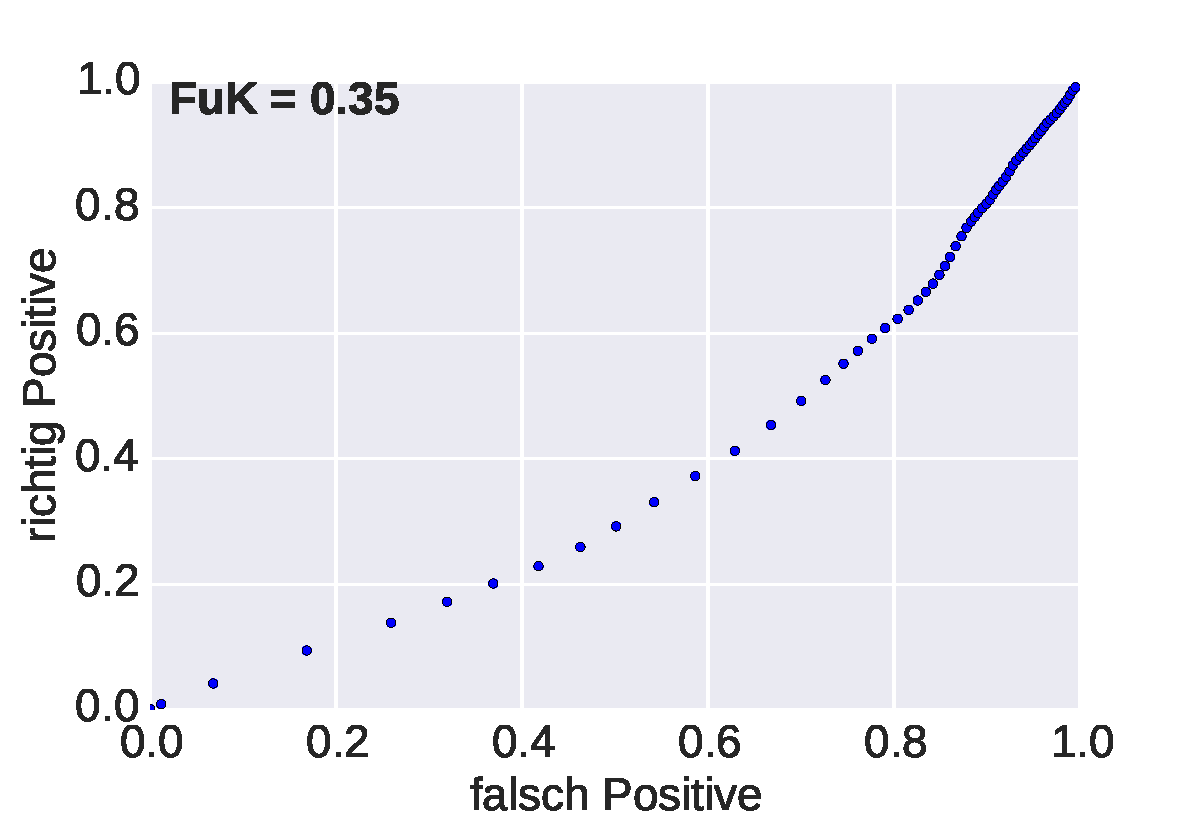
\includegraphics[height=6cm]{Abbildungen/roc_curve_E1Distanz2015albi01}}
\subfigure[Roc Kurve Elektrode 2]
{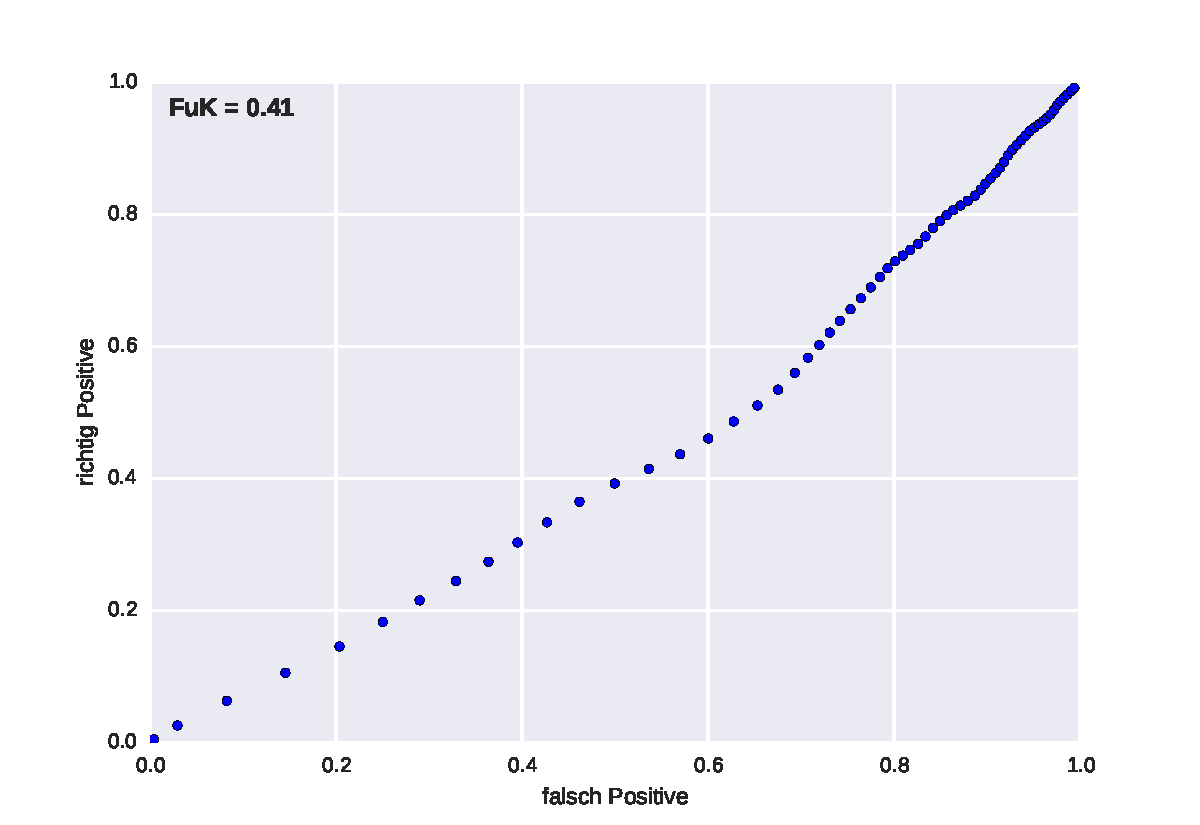
\includegraphics[height=6cm]{Abbildungen/roc_curve_E2Distanz2015albi01}}
\caption{\label{fig:roc_distanzen_entscheidung2}Roc Kurven dazu von Fisch 2}
\end{figure}




\begin{figure}[ht]
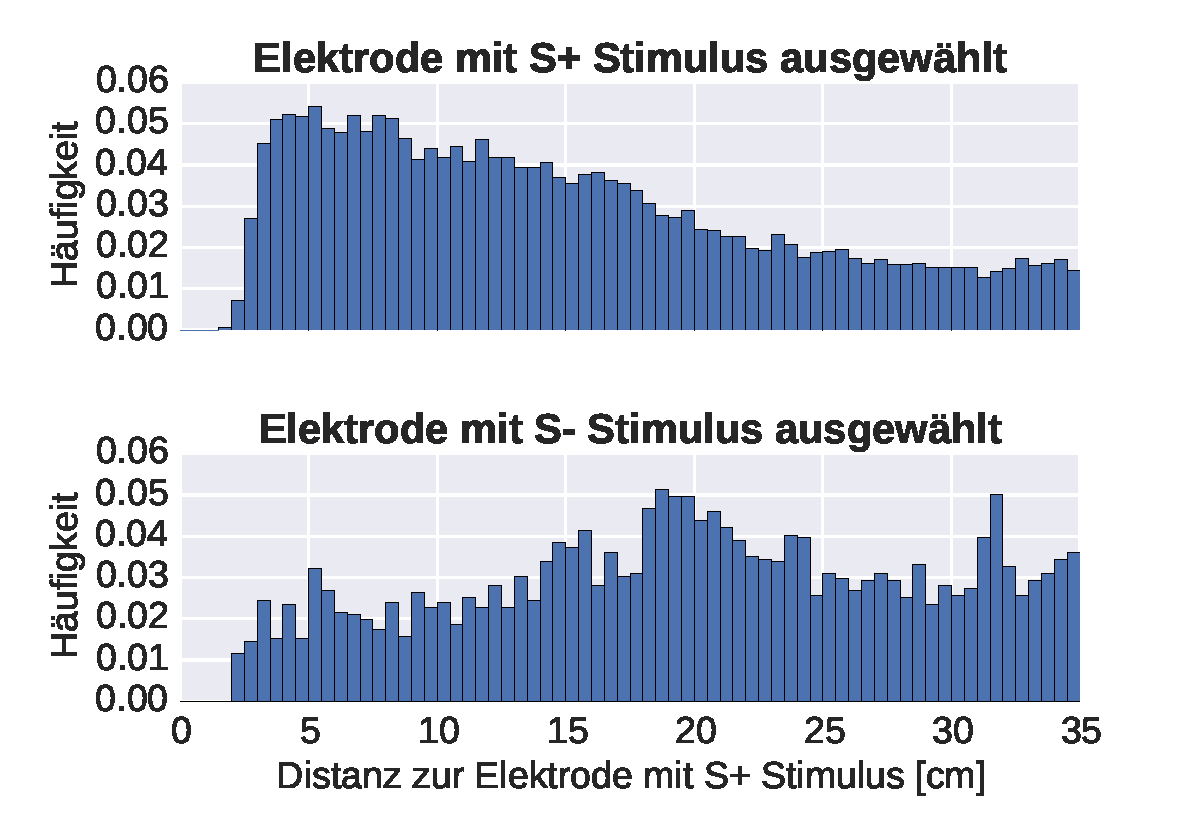
\includegraphics[height=8.5cm]{Abbildungen/Histogramm_Elektrodendistanzen3_2015albi02}
\caption{\label{fig:histodistanzen1}Fisch 1 Histogramme zur Distanz zu den Elektroden}
\end{figure}

\begin{figure}[ht]
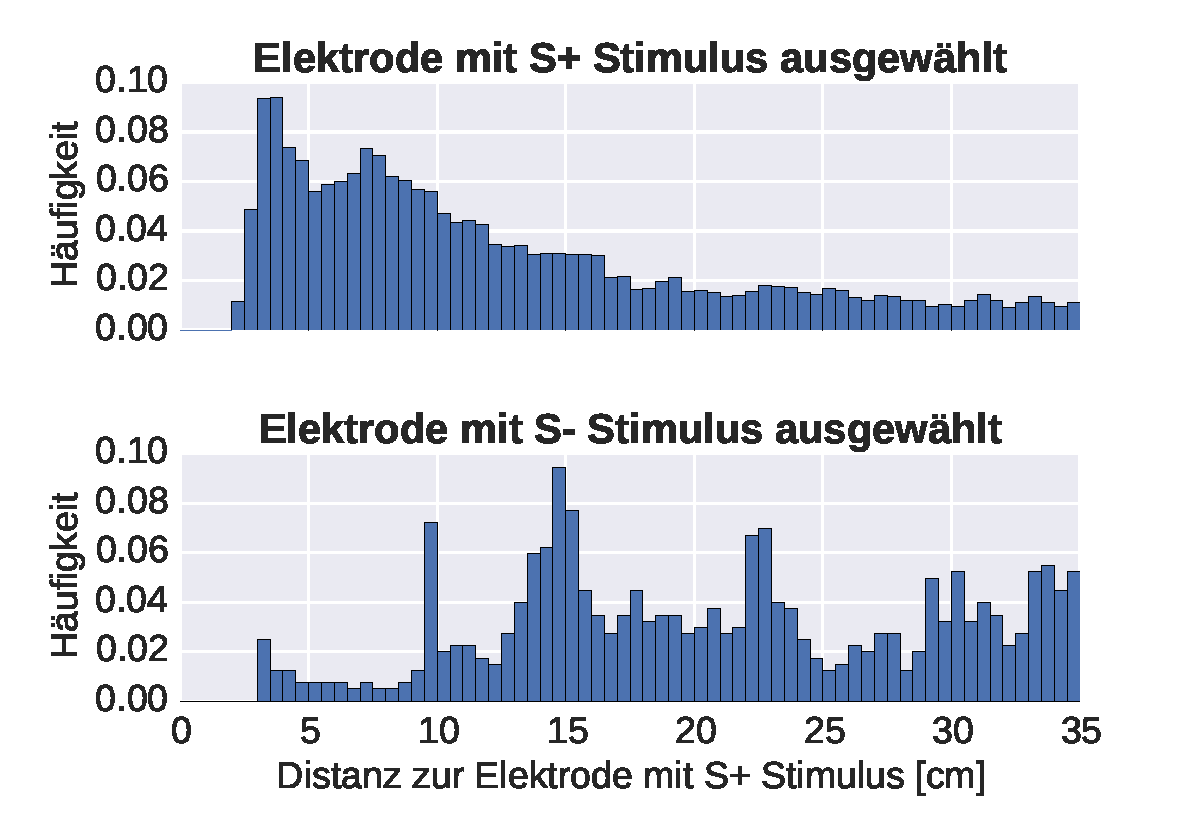
\includegraphics[height=8.5cm]{Abbildungen/Histogramm_Elektrodendistanzen3_2015albi01}
\caption{\label{fig:histodistanzen2}Fisch 2 Histogramme zur Distanz zu den Elektroden}
\end{figure}

\begin{figure}[ht]
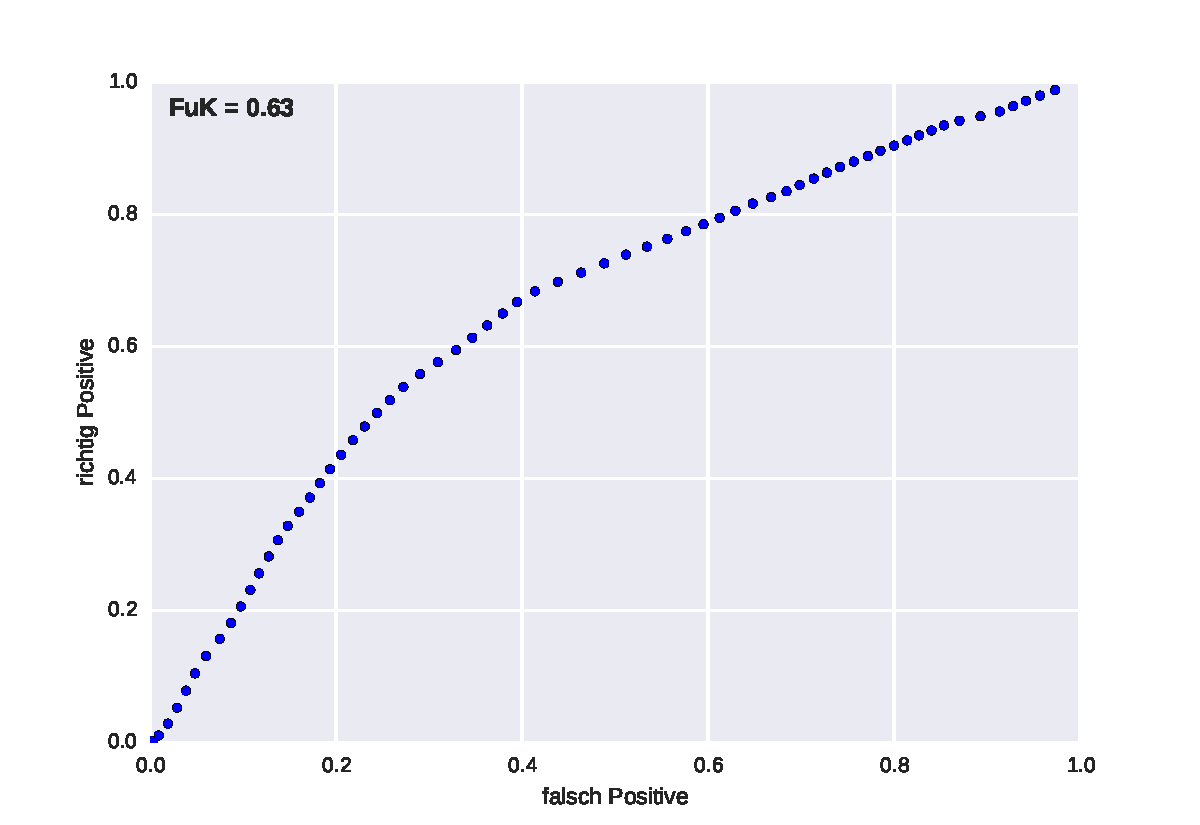
\includegraphics[height=8.5cm]{Abbildungen/roc_curve_E1Distanz22015albi02}
\caption{\label{fig:roc_distanzen1}Roc Kurven Distanzen Fisch 1}
\end{figure}


\begin{figure}[ht]
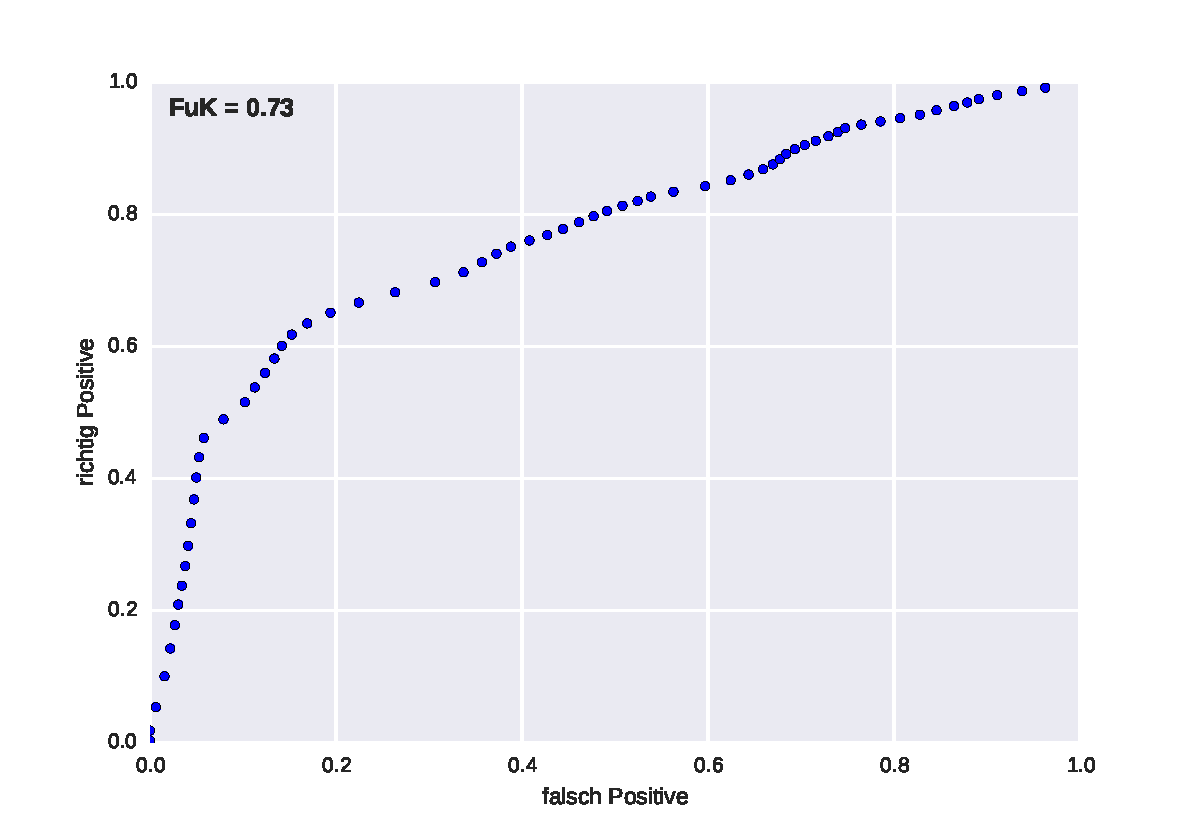
\includegraphics[height=8.5cm]{Abbildungen/roc_curve_E1Distanz22015albi01}
\caption{\label{fig:roc_distanzen2}Roc Kurven Distanzen Fisch 2}
\end{figure}

\begin{figure}[ht]
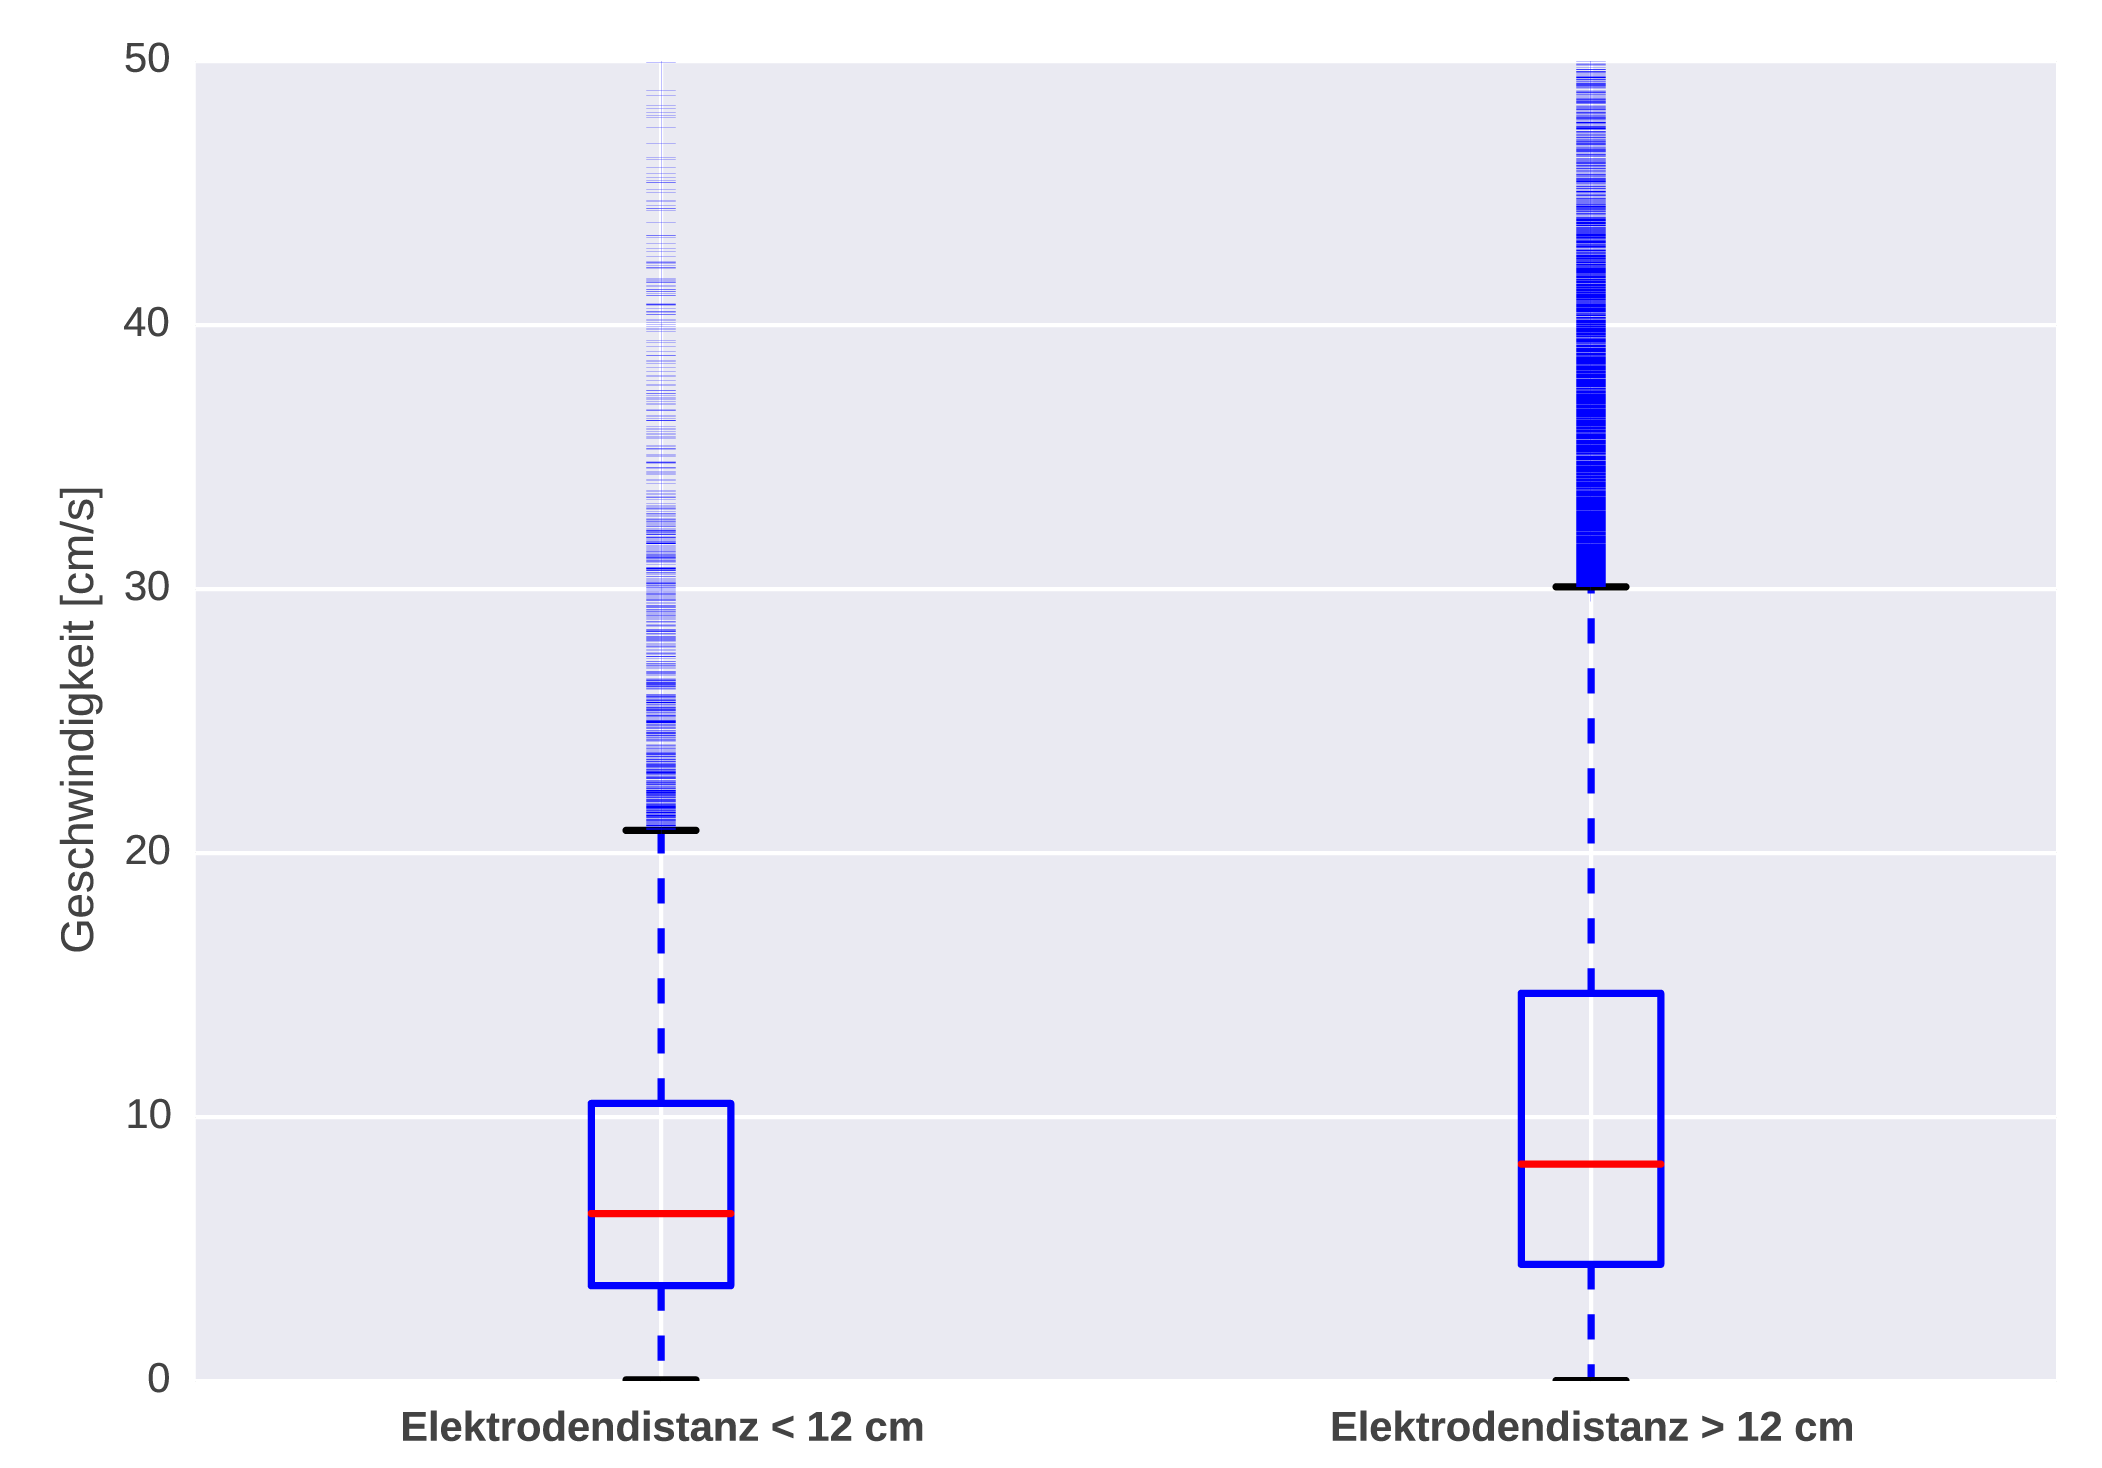
\includegraphics[height=8.5cm]{Abbildungen/Velocityboxplot2015albi02}
\caption{\label{fig: boxplot_geschwindigkeit1} Fisch 1}
\end{figure}

\begin{figure}[ht]
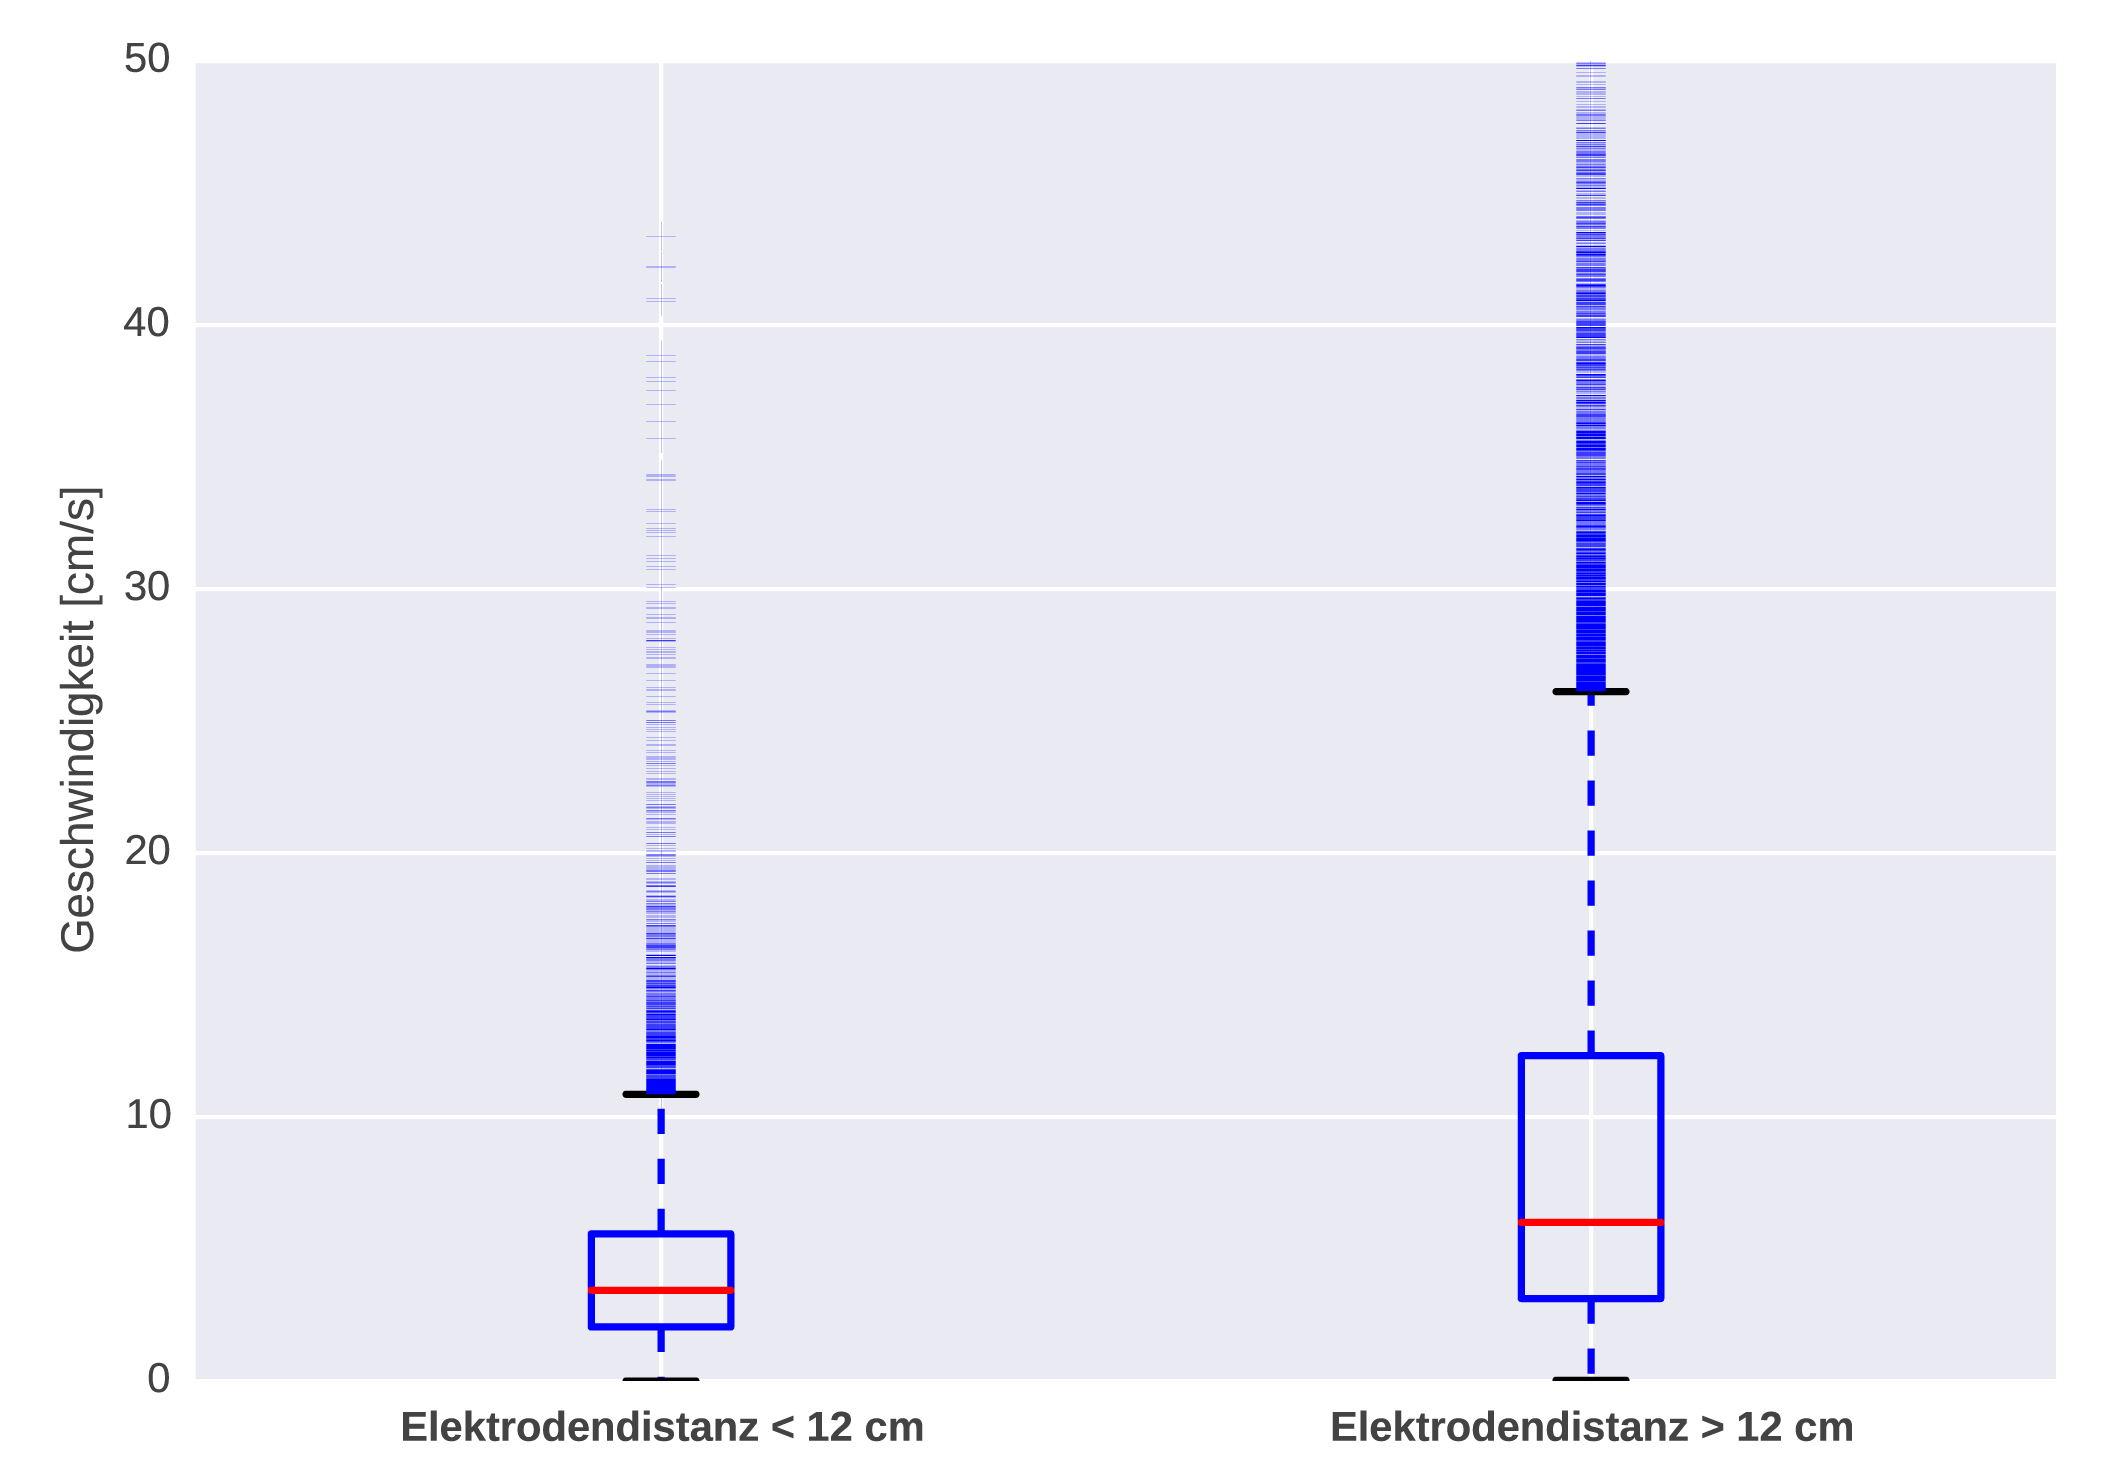
\includegraphics[height=8.5cm]{Abbildungen/Velocityboxplot2015albi01}
\caption{\label{fig: boxplot_geschwindigkeit2} Fisch 2}
\end{figure}

\begin{figure}[ht]
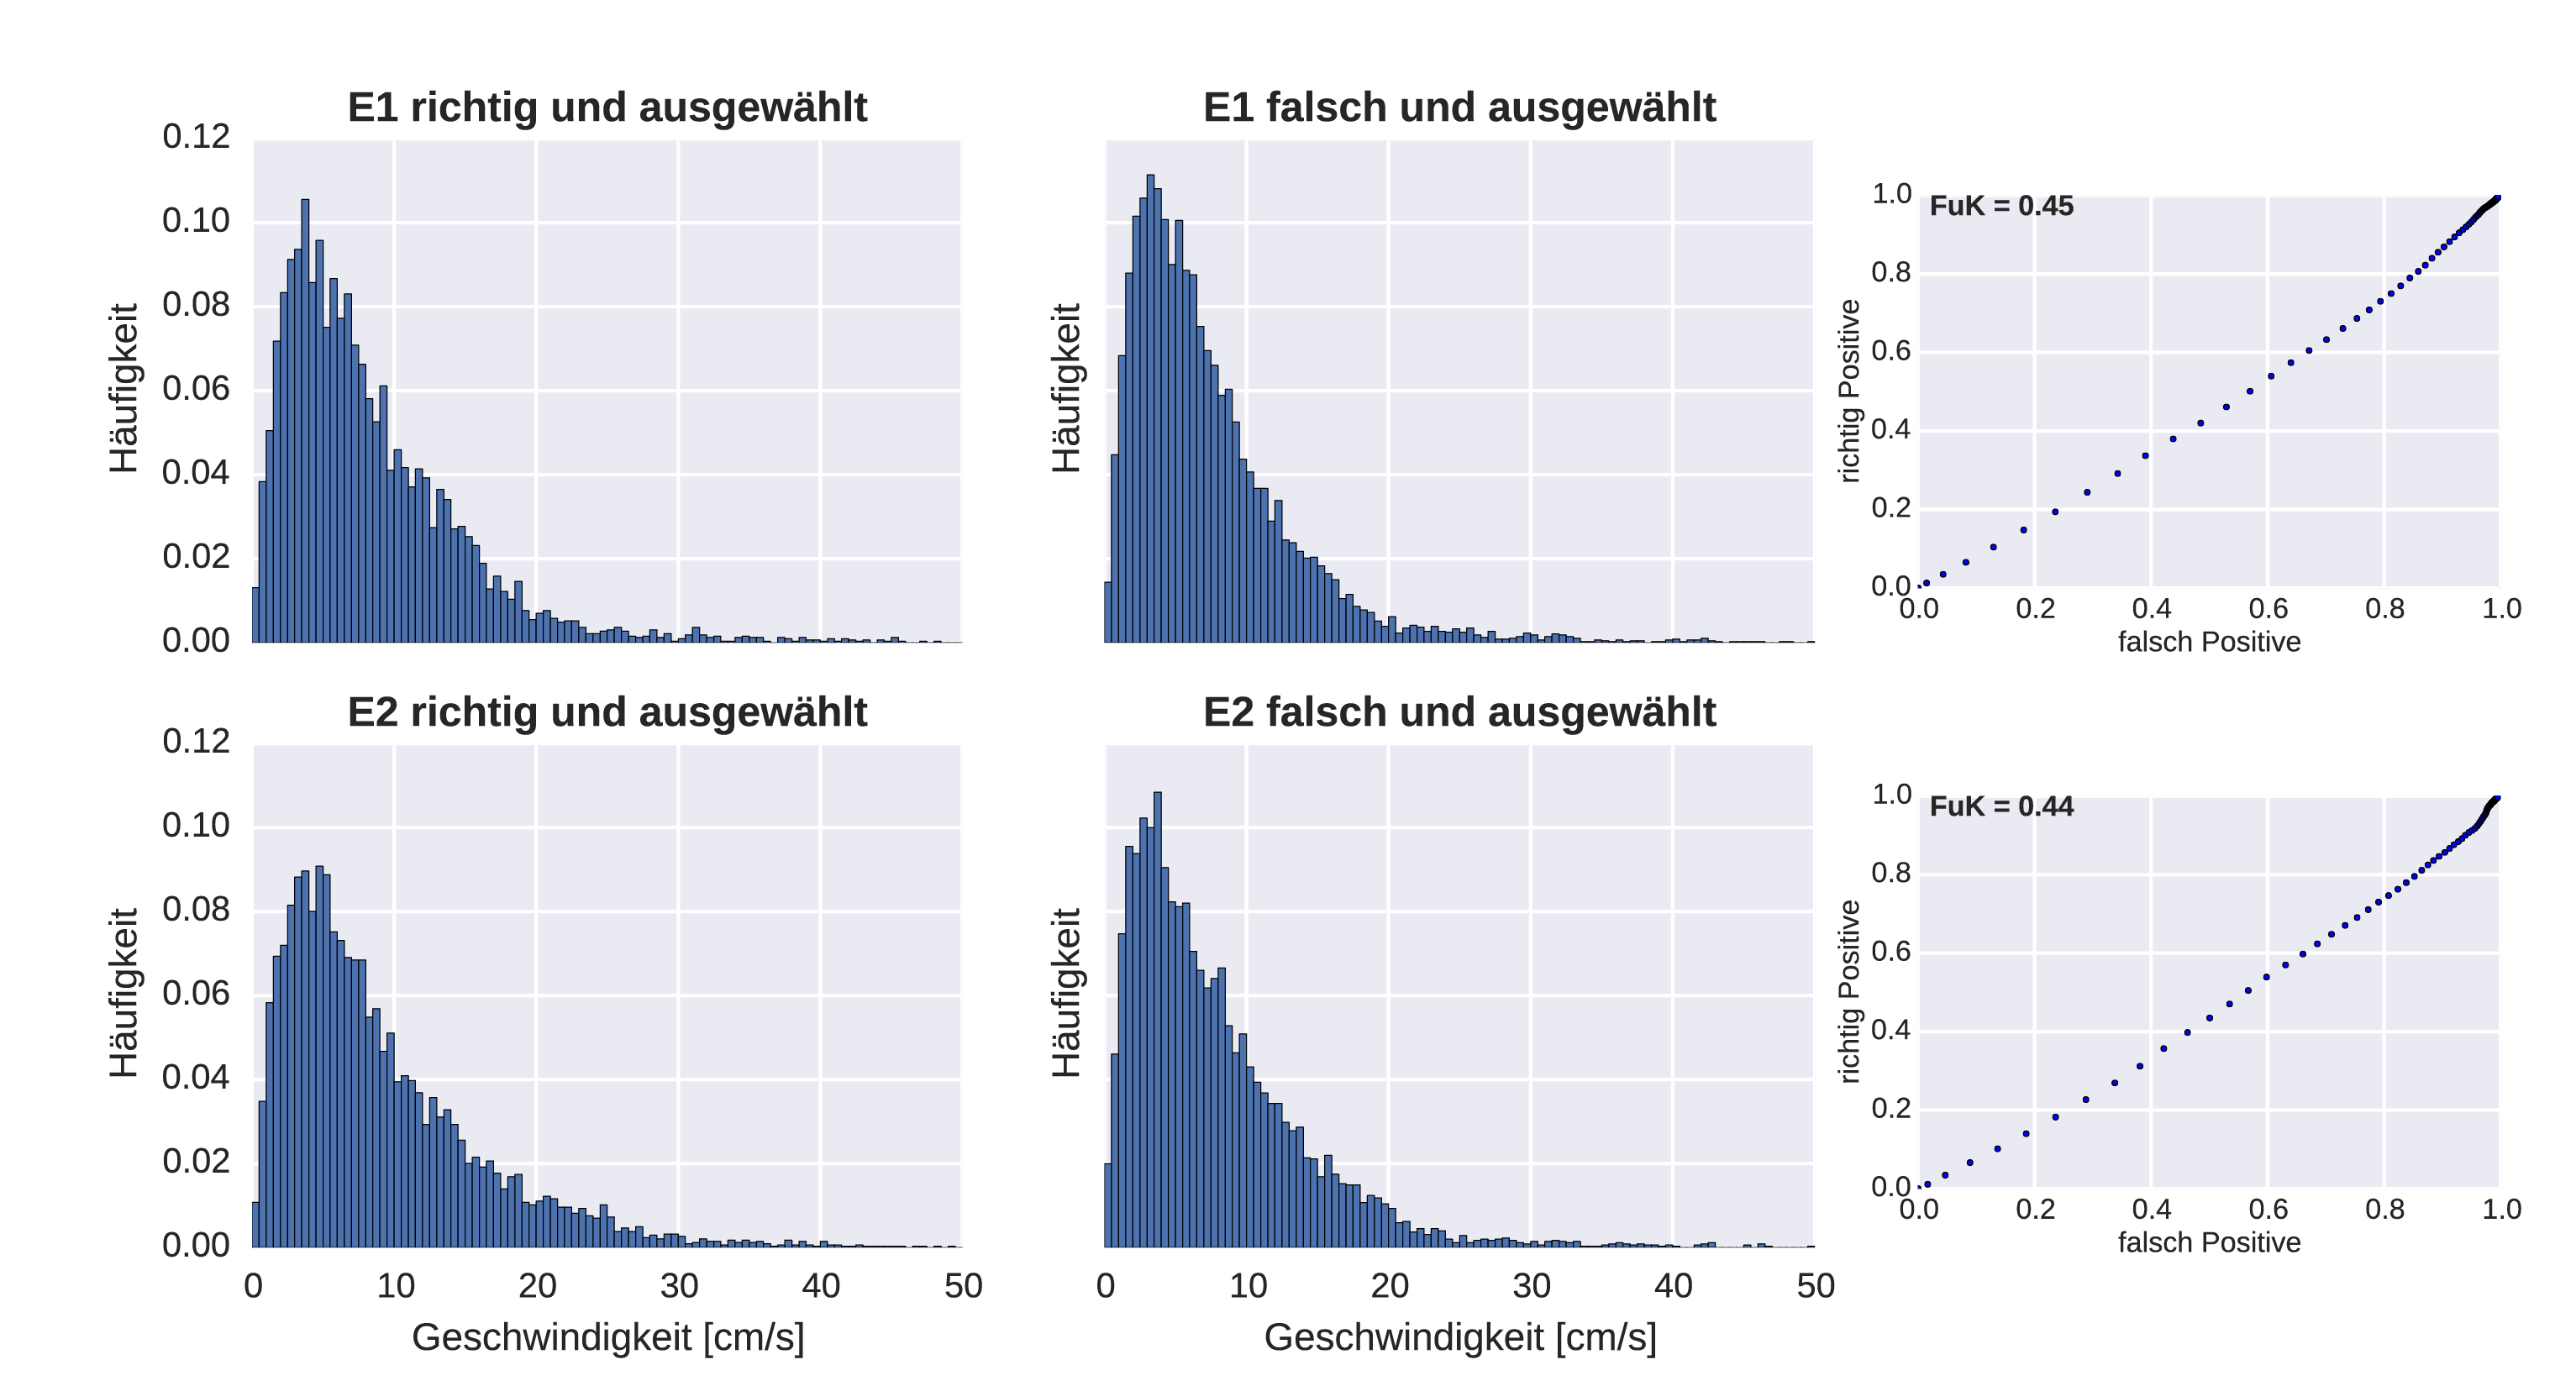
\includegraphics[height=10.5cm]{Abbildungen/Histogramm_Geschwindigkeiten_mit_Fischentscheidung2015albi02}
\caption{\label{fig: hosto_geschwindigkeit1} Fisch 1}
\end{figure}

\begin{figure}[ht]
\subfigure[Roc Kurve Elektrode 1]
{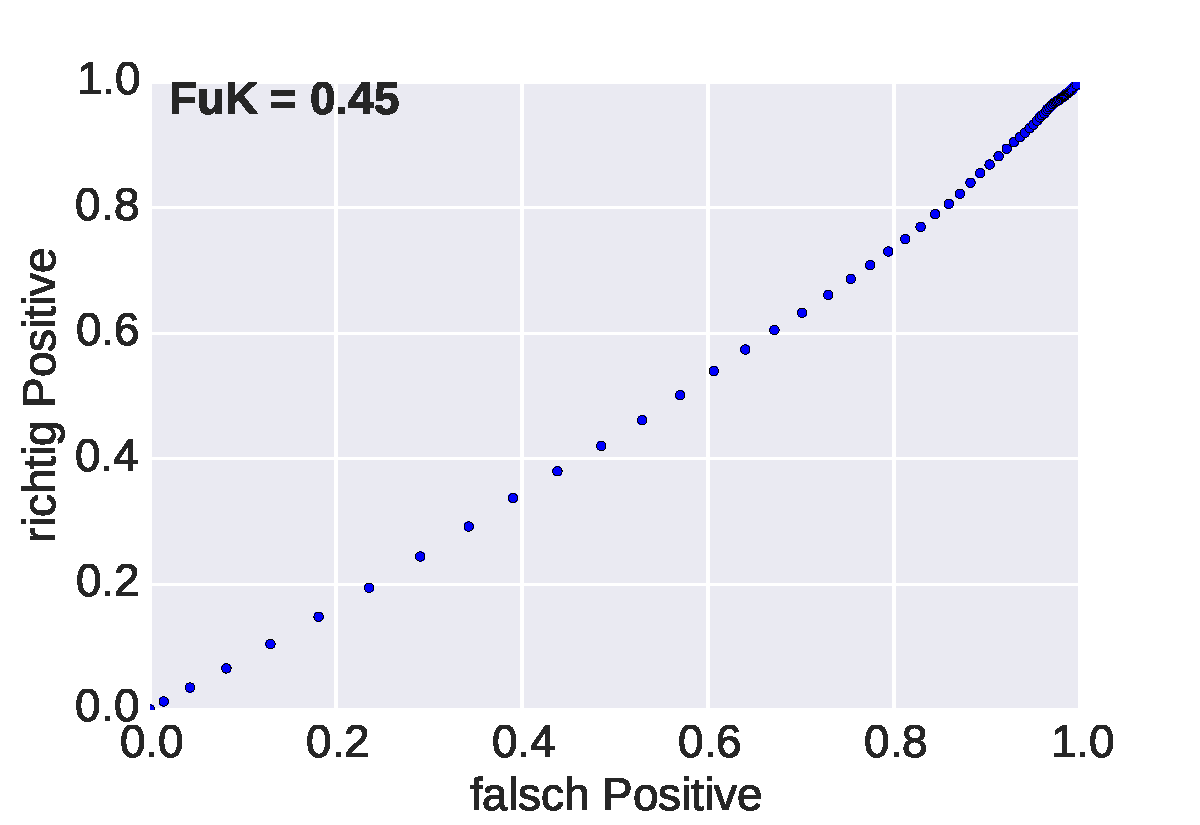
\includegraphics[height=6cm]{Abbildungen/roc_curve_E1Geschwindigkeit2015albi02}}
\subfigure[Roc Kurve Elektrode 2]
{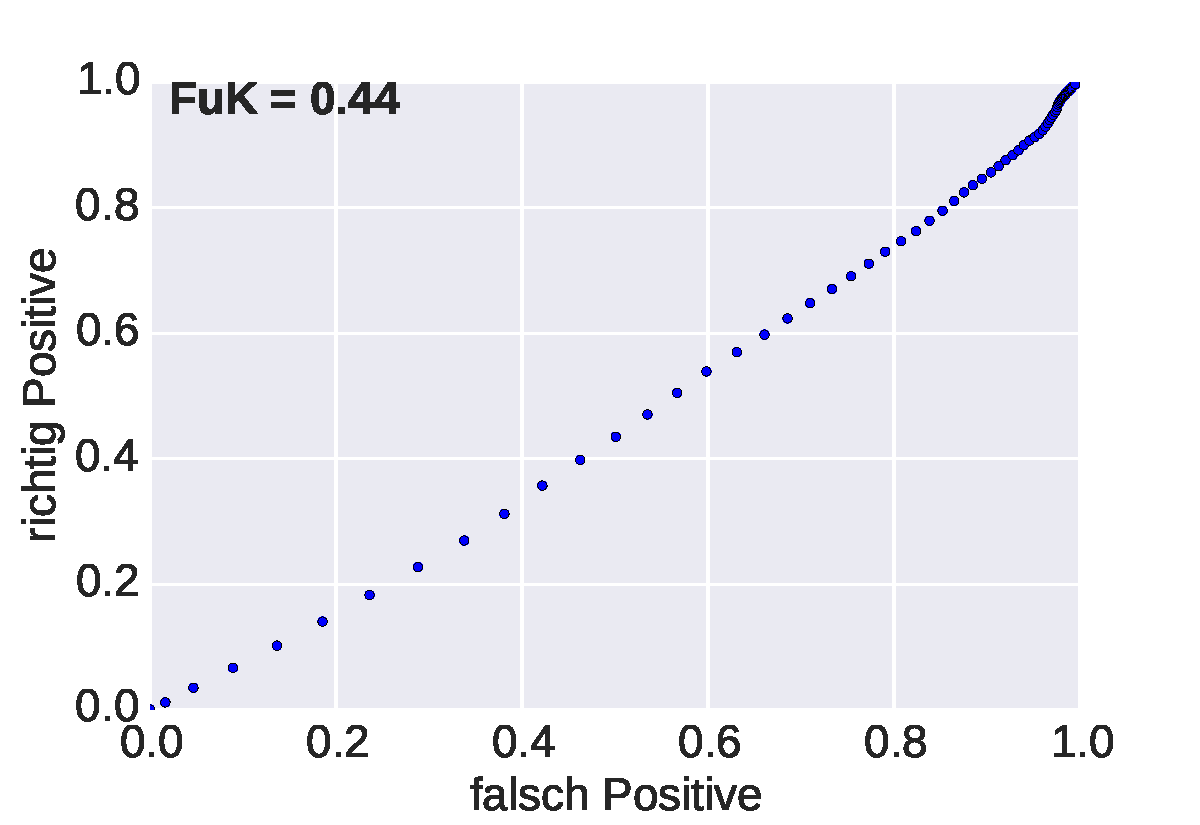
\includegraphics[height=6cm]{Abbildungen/roc_curve_E2Geschwindigkeit2015albi02}}
\caption{\label{fig:roc_geschwindigkeiten_entscheidung1}Roc Kurven Geschwindigkeiten mit Entscheidung von Fisch 1}
\end{figure}


\begin{figure}[ht]
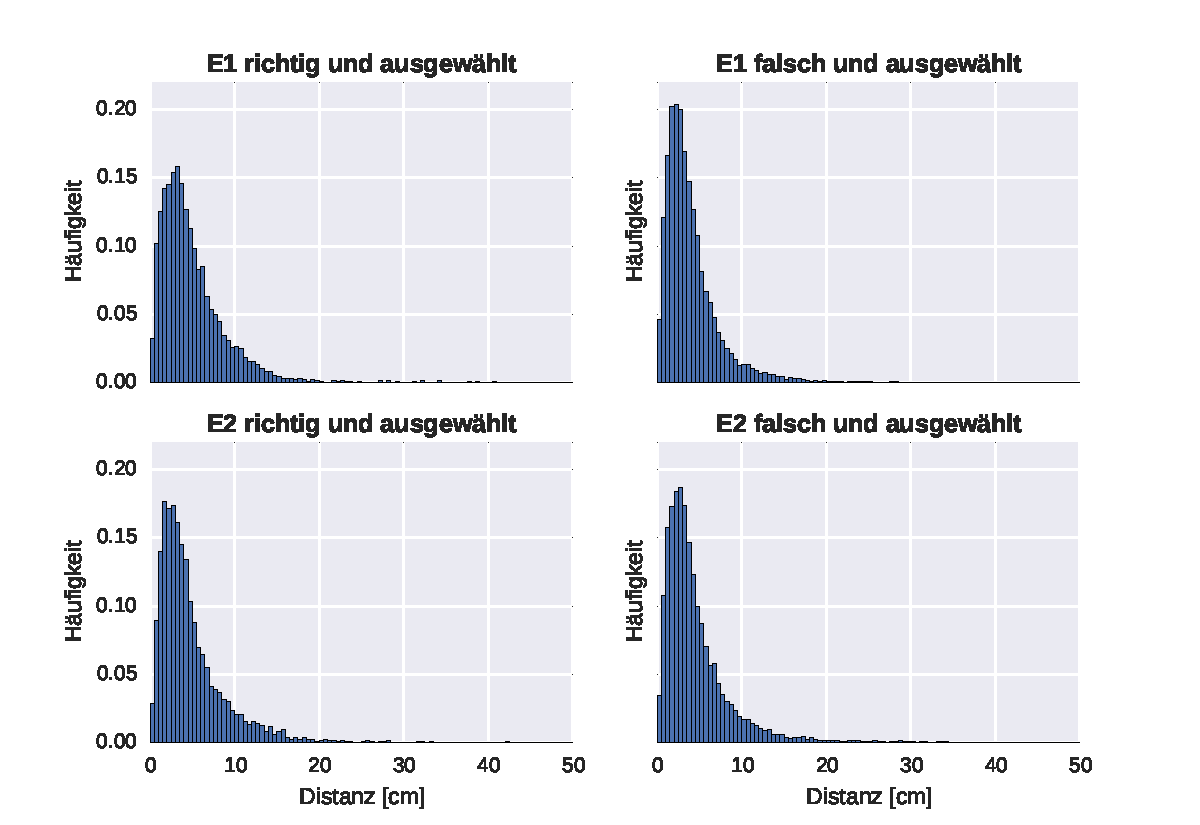
\includegraphics[height=10.5cm]{Abbildungen/Histogramm_Geschwindigkeiten_mit_Fischentscheidung2015albi01}
\caption{\label{fig: hosto_geschwindigkeit2} Fisch 2}
\end{figure}

\begin{figure}[ht]
\subfigure[Roc Kurve Elektrode 1]
{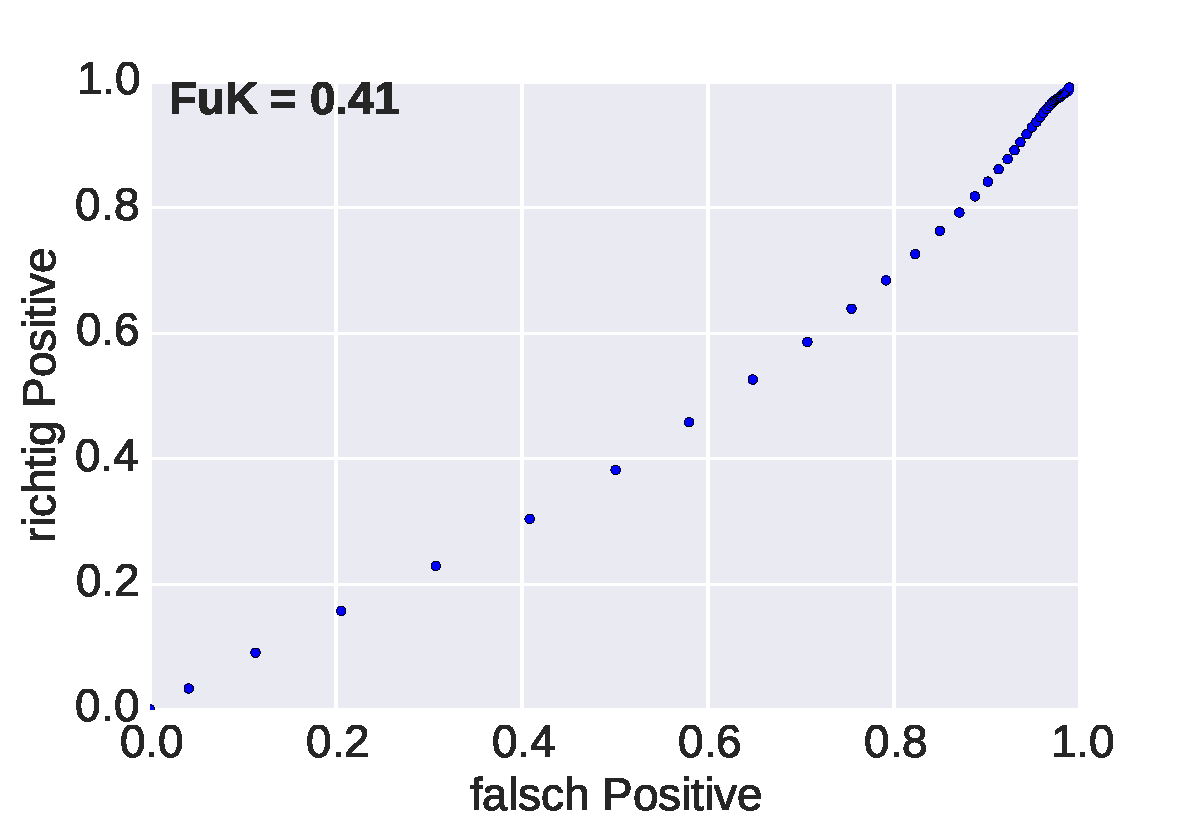
\includegraphics[height=6cm]{Abbildungen/roc_curve_E1Geschwindigkeit2015albi01}}
\subfigure[Roc Kurve Elektrode 2]
{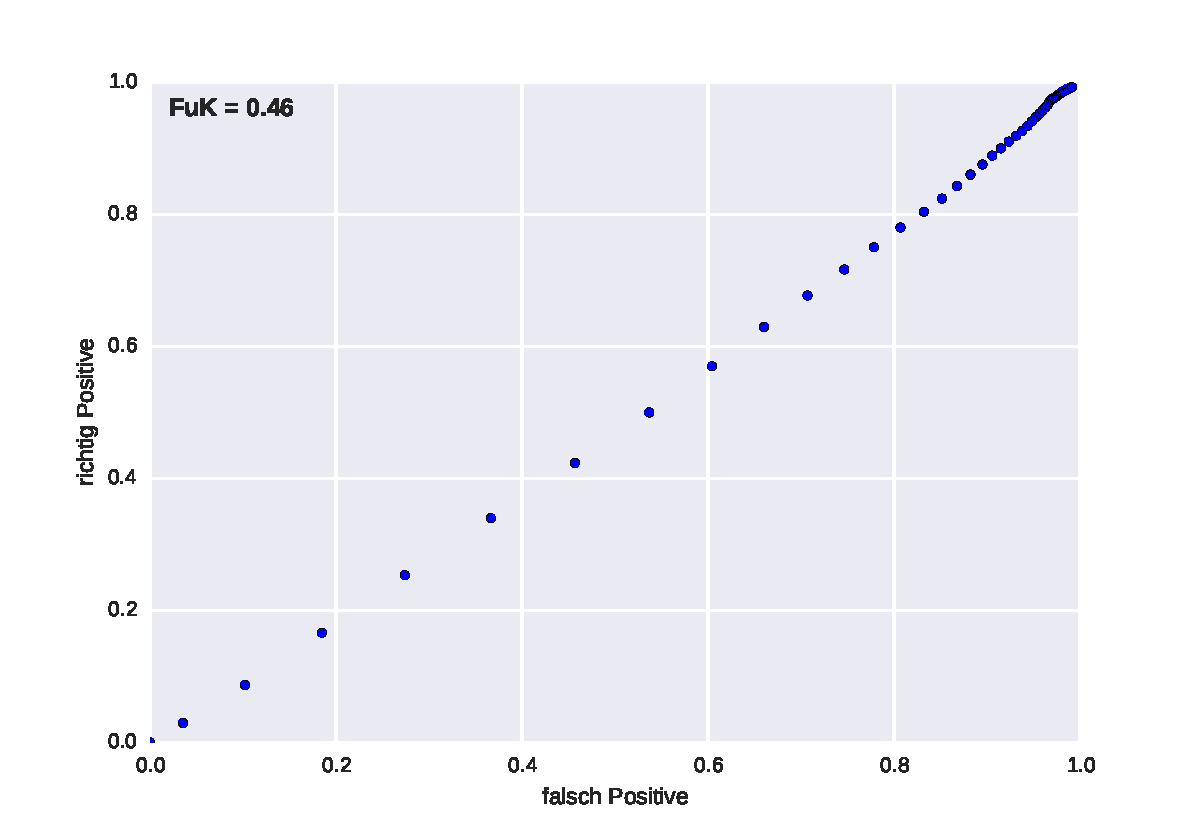
\includegraphics[height=6cm]{Abbildungen/roc_curve_E2Geschwindigkeit2015albi01}}
\caption{\label{fig:roc_geschwindigkeiten_entscheidung2}Roc Kurven Geschwindigkeiten mit Entscheidung von Fisch 1}
\end{figure}






\section{Auswertung der Vorversuche}

\subsection{Eingew�hnung}

\begin{figure}[ht]
\subfigure[Fisch 1]
{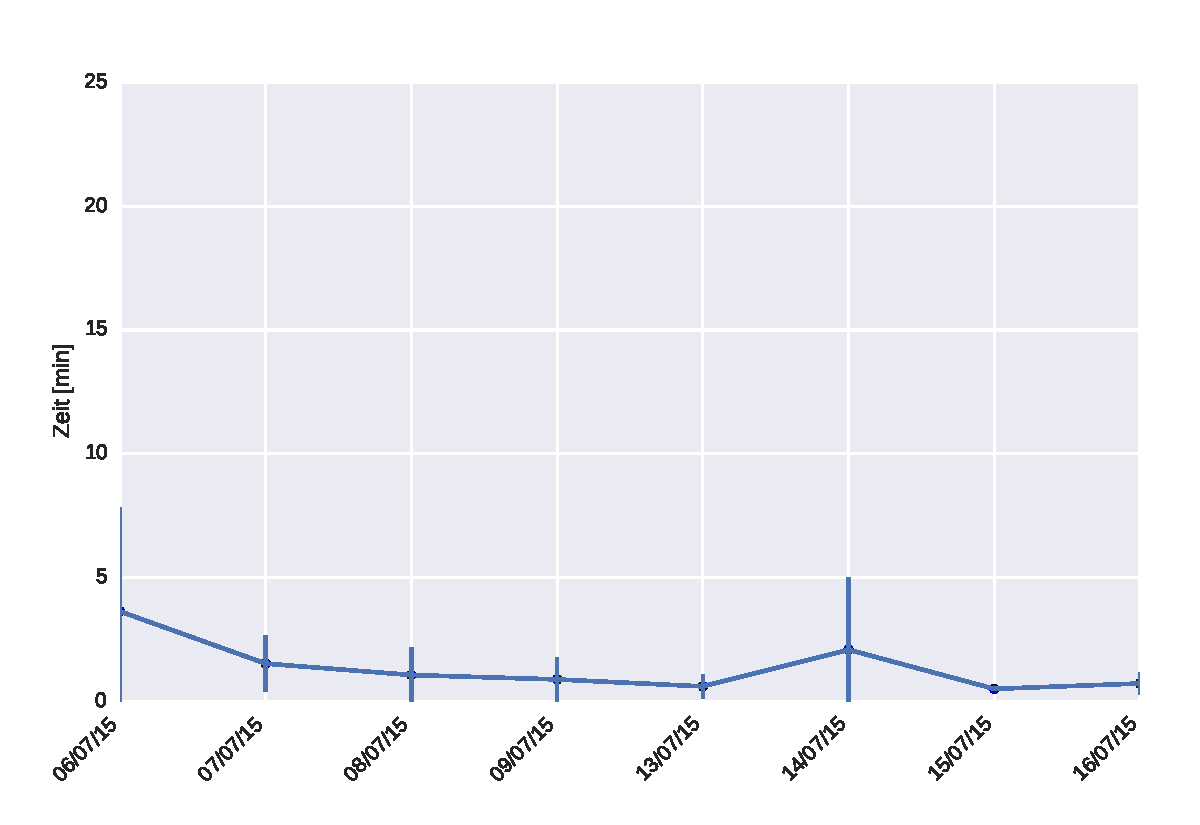
\includegraphics[height=5.5cm]{Abbildungen/date_mean_time_plot_versuch12015albi02}}
\subfigure[Fisch 2]
{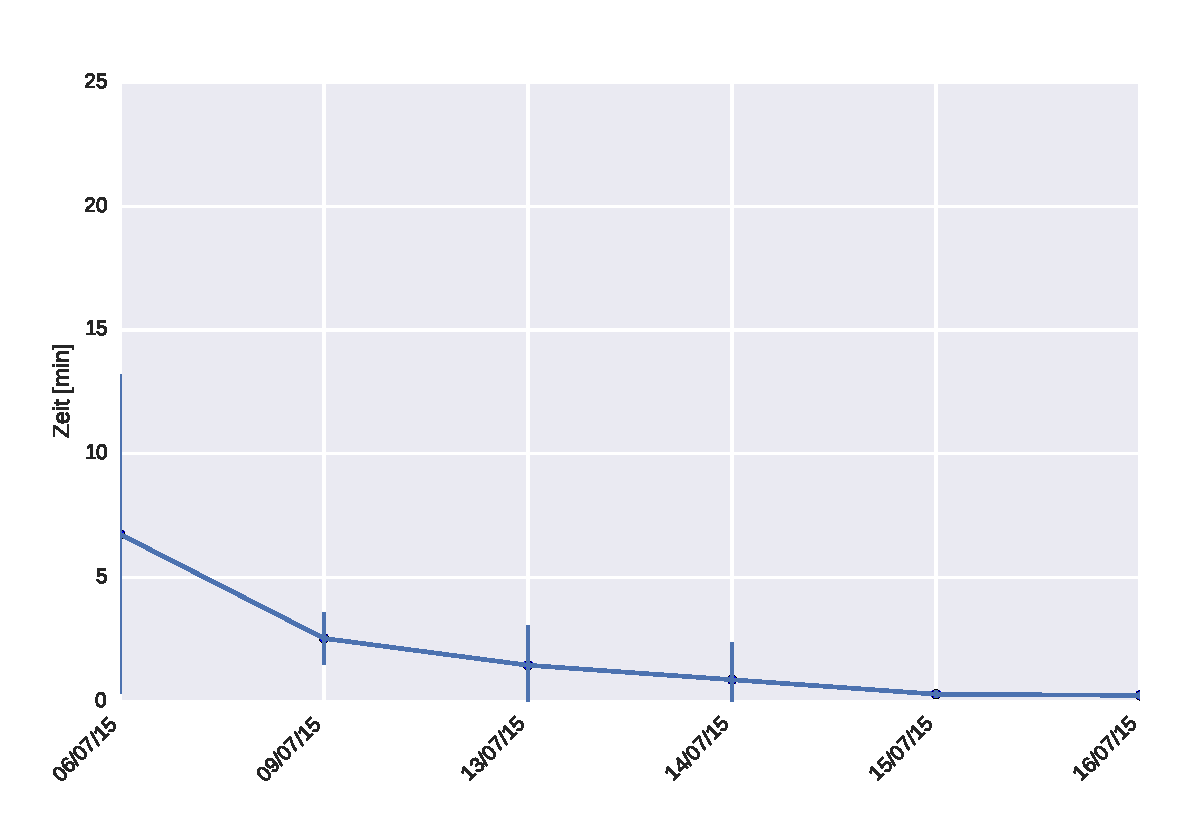
\includegraphics[height=5.5cm]{Abbildungen/date_mean_time_plot_versuch12015albi01}}
\subfigure[Fisch 3]
{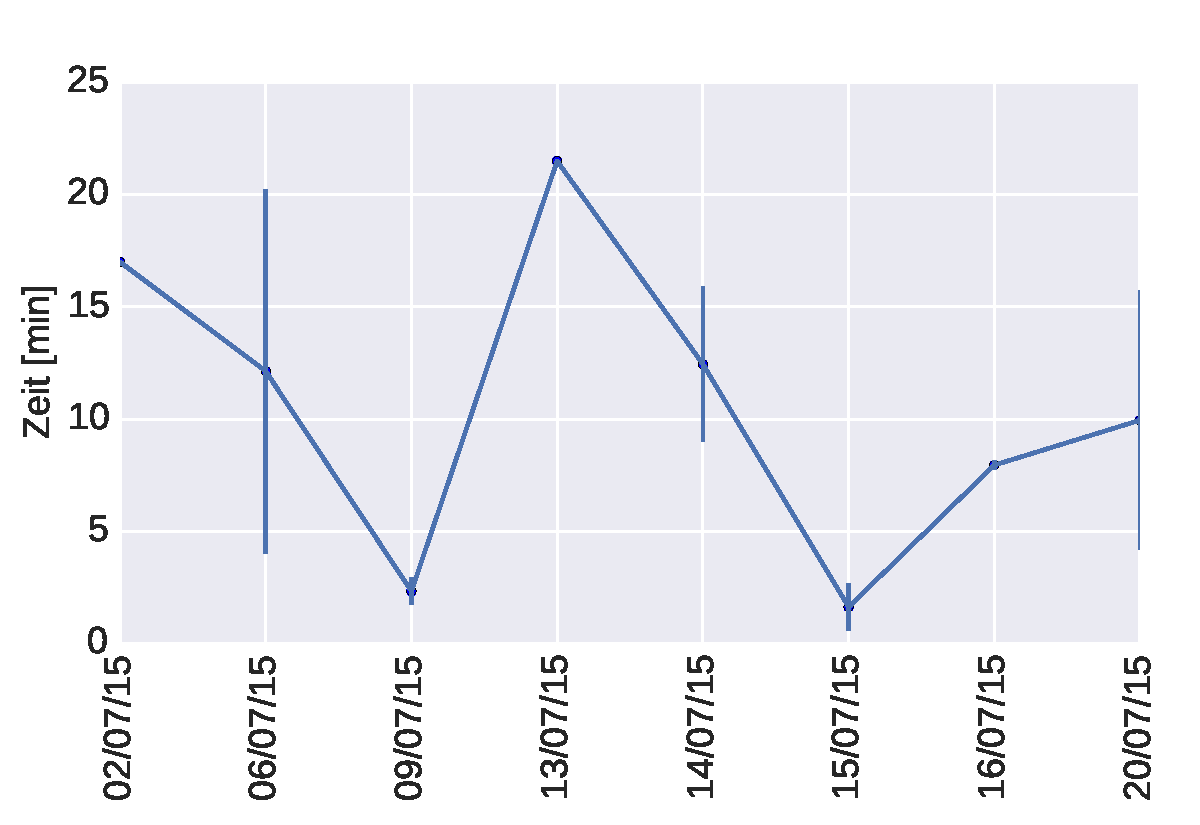
\includegraphics[height=5.5cm]{Abbildungen/date_mean_time_plot_versuch12014albi08}}
\subfigure[Fisch 4]
{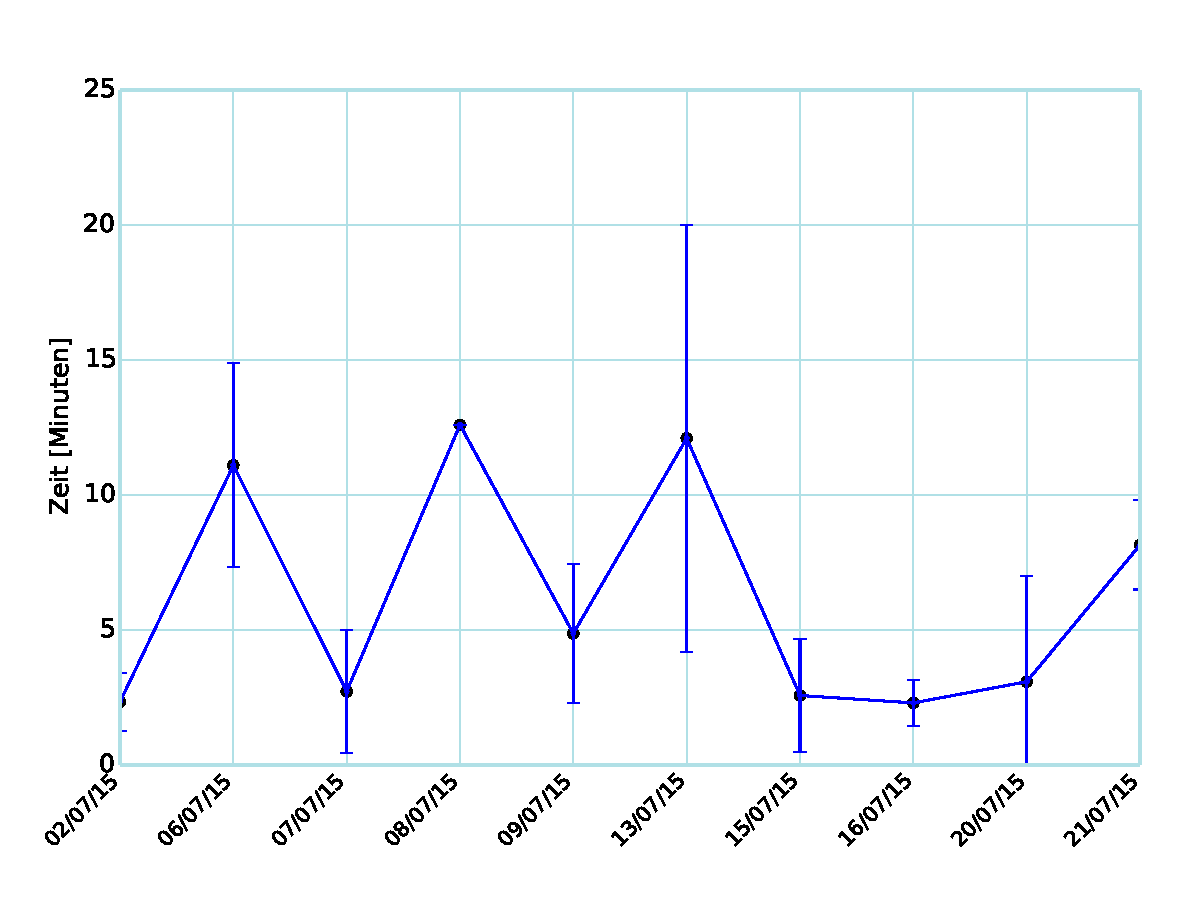
\includegraphics[height=5.5cm]{Abbildungen/date_mean_time_plot_versuch12013albi14}}
\caption{\label{fig: versuch1_zeit} Zeiten, die die Fische gebraucht haben um den Versuch erfolgreich zu beenden.}
\end{figure}
